% THIS DOCUMENT IS FOLLOWS THE VOLERE TEMPLATE BY Suzanne Robertson and James Robertson
% ONLY THE SECTION HEADINGS ARE PROVIDED
%
% Initial draft from https://github.com/Dieblich/volere
%
% Risks are removed because they are covered by the Hazard Analysis
\documentclass[12pt]{article}

\usepackage{fullpage}
\usepackage{booktabs}
\usepackage{tabularx}
\usepackage{longtable}
\usepackage{graphicx}
\usepackage{float}
\usepackage{amsmath,amssymb}
\usepackage{tikz}
\usetikzlibrary{positioning,arrows.meta,shapes.geometric,fit,calc}
\usepackage{hyperref}
\hypersetup{
    bookmarks=true,         % show bookmarks bar?
      colorlinks=true,      % false: boxed links; true: colored links
    linkcolor=red,          % color of internal links (change box color with linkbordercolor)
    citecolor=green,        % color of links to bibliography
    filecolor=magenta,      % color of file links
    urlcolor=cyan           % color of external links
}

\setlength{\emergencystretch}{3em}

\newcommand{\lips}{\textit{Insert your content here.}}

\input{../Comments.text}
\input{../Common.text}

\begin{document}

\title{Software Requirements Specification\\\progname}
\author{\authname}
\date{}
	
\maketitle

~\newpage

\pagenumbering{roman}

\tableofcontents

~\newpage

\section*{Revision History}

\begin{tabularx}{\textwidth}{p{3cm}p{2cm}X}
\toprule {\textbf{Date}} & {\textbf{Version}} & {\textbf{Notes}}\\
\midrule
Oct 18, 2026 & 0.1 & Draft requirements for the current Tandem scope.\\
Oct 19, 2026 & 0.2 & Make source-to-target KV cache prediction central to the scope, requirements, evaluation and workflow diagram.\\
Oct 19, 2026 & 0.3 & Shorten supporting sections and requirements; mark host-provided security features not applicable and consolidate duplicate checks.\\
Oct 20, 2026 & 0.4 & Present functional and quality requirements as bullet points; replace most mathematical notation with plain-language checks.\\
Oct 20, 2026 & 0.5 & Remove the traceability matrix and draft test-settings table; replace remaining setting references with plain-language limits.\\
Nov 20, 2026 & 0.6 & Restore named test settings with values, units, reasons and draft status in an appendix.\\
Nov 21, 2026 & 1.0 & Address the grading and peer-review feedback: add SR-09 to SR-15 and FR-17 from the Hazard Analysis; split NFR-05 into same-model and cross-model checks; restore the traceability matrix with priorities and a phase-in plan; redraw the figures in UML; list rules and assumptions with reasons; clarify ambiguous requirements.\\
\bottomrule
\end{tabularx}

~\\

~\newpage
\pagenumbering{arabic}
\section{Purpose of the Project}


\subsection{User Business}
Tandem predicts a target large language model's key-value (KV) cache from a
source model's KV cache to avoid repeating prefill for shared conversation
history after a model switch. The intended benefits are lower GPU compute,
serving cost and time to first token (TTFT).

vLLM Semantic Router selects the target model.
Tandem validates and loads the prediction; the engine prefills the uncached
suffix and decodes. Unsupported or failed predictions use native processing.
The project includes predictor development, any fitting/training, paired KV
data and engine integration on one GPU server; base LLM weights stay frozen.
Accuracy and end-to-end benefits remain to be demonstrated.


\subsection{Goals of the Project}
Tandem addresses repeated prefill after model switches:
\begin{description}
\item[G1: Predict target KV from source KV.] Develop and integrate a predictor
that lets supported target models reuse the shared history without repeating
prefix prefill.
\item[G2: Reduce compute and serving cost.] Lower GPU time per completed
request after counting prediction, validation and cache-loading overhead.
\item[G3: Support economical model switching.] Preserve the benefit of routing
suitable requests to cheaper models by reducing repeated history processing.
\item[G4: Improve latency and throughput.] Lower time to first token (TTFT)
and increase completed requests per second within the agreed latency limits.
\end{description}
Matched native/Tandem tests measure KV error, output effects, actual prompt
work, GPU time, latency and throughput. Cost claims state rates and assumptions;
router-selection savings are reported separately. Output accuracy, privacy
and native fallback remain required.


\section{Stakeholders}


\subsection{Client}
A potential client is a multi-model application company such as
Cursor, whose team could help identify useful
model combinations, acceptable response delays and cost-saving goals; this
is a proposed adoption scenario, not a confirmed partnership.


\subsection{Customer}
A potential customer is an inference provider such as
Together AI or an internal AI infrastructure
team that could deploy Tandem to serve more requests with its GPUs; adoption
of the planned open-source software does not require a licence purchase.


\subsection{Other Stakeholders}
Other people who could benefit include:
\begin{itemize}
\item \textbf{Independent application developers looking to host local LLM:} could provide faster
AI features without needing to build their own serving optimization.
\item \textbf{Inference Data Center Operators:} could make better use of limited GPU capacity
and see clear information about cache reuse and failures.
\item \textbf{Researchers:} could use the test tools and results to study
when sharing cached calculations is useful and when it is ineffective.
\end{itemize}

\subsection{Hands-On Users of the Project}
Engine developers integrate the predictor; operators configure approved
predictors and resource limits; researchers evaluate results; application
developers use the existing serving interface. Technical users need Linux,
LLM-serving and GPU knowledge. vLLM Semantic Router selects the target model,
and application end users need no knowledge of Tandem.


\subsection{Personas}
These are potential adoption scenarios, not confirmed partnerships or
company-supplied requirements; Alex Morgan and Sofia Nguyen are fictional.

\par\medskip\noindent\phantomsection\label{persona:cursor}
\textbf{Cursor (AI Application Company).}
Cursor offers multi-model AI development tools.
In this scenario, coding conversations retain instructions, code and earlier
responses across model switches. The application team wants cheaper model
choices without repeated history prefill erasing the savings. Tandem would
require a compatible backend with KV access; a hosted API alone is insufficient.
The team needs documented model pairs, unchanged prompts and routing,
measured benefits and native fallback.

\par\medskip\noindent\phantomsection\label{persona:together}
\textbf{Together AI (Inference Hosting Provider).}
Together AI offers dedicated inference.
This scenario represents operators managing GPU capacity, queues and customer
isolation. They would configure approved predictors, model pairs and limits,
monitor reuse and failures, and disable prediction when needed. Adoption
requires accuracy/privacy checks and gains that include prediction/loading
overhead; production-stack compatibility needs separate assessment.

\par\medskip\noindent\phantomsection\label{persona:alex}
\textbf{Alex Morgan (Inference-Engine Maintainer).}
Alex maintains a vLLM deployment using Python and GPU tensor operations.
Frequent model and dependency updates can break cache integration. Alex needs
versioned interfaces and tests covering prediction, validation, loading,
suffix prefill and decoding, plus diagnostics for unsupported caches and
reliable native fallback.

\par\medskip\noindent\phantomsection\label{persona:sofia}
\textbf{Sofia Nguyen (LLM Inference Researcher).}
Sofia studies efficient LLM serving on shared laboratory GPUs. She compares
predicted and native KV state and measures when prediction overhead outweighs
saved prefill. She needs held-out conversations, matched routing/settings,
repeated trials, output checks, cache/fallback records and reproducible
hardware/software details. Measured GPU time and estimated monetary savings
must remain distinguishable.


\subsection{Priorities Assigned to Users}
Output accuracy and privacy take priority, followed by reliable fallback,
lower inference cost and latency, higher capacity and reproducible evidence;
these priorities apply across the four personas.


\subsection{User Participation}
Potential application developers, operators, maintainers and researchers can
review integration examples, recovery scenarios and benchmarks; record actual
participants and feedback separately from the hypothetical personas.


\subsection{Maintenance Users and Service Technicians}
Alex Morgan represents integration maintenance and Together AI represents
operational support; both need versioned setup instructions and diagnostics,
while the hosting organization maintains hardware, access and the operating system.


\section{Mandated Constraints}


\subsection{Solution Constraints}
The initial project has these limits:
\begin{description}
\item[C1:] Run text-generation requests on one server.
\item[C2:] Use the target model selected by vLLM Semantic Router, or the same
recorded routing decision when replaying a benchmark.
\item[C3:] Use existing trained source and target LLMs with frozen base-model
weights. Developing a KV cache predictor, including fitting or training its
parameters if the chosen method requires it, is part of Tandem.
\item[C4:] Reuse only an exact matching start of the conversation, using a
model pair and KV prediction method that have passed the required tests.
\item[C5:] Keep the serving engine's normal prompt processing available
whenever reuse is not possible.
\end{description}
These limits keep the project manageable and allow a fair comparison with the
serving engine running without Tandem.

\subsection{Implementation Environment of the Current System}
Use a Linux GPU server with sufficient model memory, with vLLM as the planned
engine and SGLang as an alternative; record exact model,
tokenizer, engine and GPU-software versions before testing. CPU checks do not
establish GPU performance. The proof-of-concept pair is SmolLM2-360M-Instruct
(source) and Qwen2.5-0.5B-Instruct (target), run on Hugging Face Transformers.


\subsection{Partner or Collaborative Applications}
The application sends conversation messages and generation settings through
the existing serving interface; vLLM Semantic Router selects the target. The engine supplies source KV through an internal
cache reference, not HTTP tensor uploads.
Tandem predicts and validates target KV, loads accepted state and prefills the
uncached suffix. The full prompt remains available for checks and fallback.
Native target KV references are computed offline for development/evaluation,
not as hidden shared-prefix prefill during serving. The application retains
conversation storage and access control; benchmarks replay routing decisions.


\subsection{Off-the-Shelf Software}
Reuse the serving engine, Python, PyTorch, Hugging Face Transformers,
tokenizers and GPU libraries; record versions/licences and rerun compatibility
tests after relevant updates. Predictor training is in scope; base-LLM training is not.


\subsection{Anticipated Workplace Environment}
Develop locally and use a shared Linux GPU server for model experiments,
recording hardware and competing workloads for repeatable performance tests.


\subsection{Schedule Constraints}
The Development Plan schedules the SRS/Hazard Analysis for October 19, 2026,
proof of concept in November, initial demonstration in February and final
work in March--April; confirm course dates and reconcile scope under OI5
(see Section~\ref{sec:phases}).


\subsection{Budget Constraints}
Use existing university GPU resources; available compute time and storage
remain unconfirmed (OI7), so reschedule or reduce tests if resources are insufficient.


\subsection{Enterprise Constraints}
Review repository changes through issues and pull requests, record release
versions, and keep credentials and private conversations out of public files;
use only public, synthetic or permitted test data.


\section{Naming Conventions and Terminology}


\subsection{Glossary of All Terms, Including Acronyms, Used by Stakeholders
involved in the Project}
\begin{longtable}{@{}p{0.25\textwidth}p{0.69\textwidth}@{}}
\toprule Term & Meaning\\\midrule\endhead
LLM & Large language model; generates text.\\
Inference & Running a trained model to produce output.\\
Semantic routing & Selecting a target model from request needs and policy; the planned router is vLLM Semantic Router.\\
Serving engine & Software that loads models, schedules requests and returns responses.\\
Source/target model & The model supplying existing KV state / the router-selected model receiving predicted KV state.\\
Token/tokenizer & A unit of text / the converter between text and token IDs.\\
Prefill & Processing prompt tokens to compute attention state before generation.\\
Decoding & Generating response tokens while extending the KV cache.\\
Attention & Combining contextual information using query, key and value tensors.\\
Tensor & A multidimensional numeric array.\\
KV cache & Stored attention-layer key/value tensors for processed tokens.\\
Source KV cache & The earlier model's KV tensors for a recorded prefix.\\
Cache handle & A reference to engine-managed KV tensors.\\
Uncached prompt suffix & All tokens after the cached prefix; still requires target prefill.\\
KV cache predictor & A versioned mapping from source KV to estimated target KV, possibly fitted/trained.\\
Predicted target KV cache & Estimated target attention state; accuracy requires evaluation.\\
Native reference KV cache & Target KV computed by normal prefill for offline ground truth.\\
Cache provider / loading component & Trusted engine-side code retrieving source KV and loading accepted predictions.\\
Cross-model KV reuse & Replacing target-prefix prefill with KV predicted from source KV.\\
Prefix caching & Reusing KV for an exact shared prompt prefix.\\
Candidate cache & Predicted target KV awaiting runtime validation.\\
Target-ready cache & KV in the target layout; this alone does not establish accuracy.\\
Context prefix & The exact shared start of a conversation in target-model tokens.\\
Native prefill & Standard prompt processing, including available native prefix caching.\\
Native processing / baseline & The engine without Tandem, retaining its existing cache features.\\
Fallback & Returning to native processing when prediction/reuse cannot be used.\\
Compatibility manifest & Versioned list of qualified model pairs, predictors and settings.\\
Profile / qualification & A model/cache setup / its required approval tests.\\
Reuse domain & Host-assigned group permitted to share specified history.\\
Cold/warm cache & No useful saved prefix / a relevant cached prefix.\\
TTFT & Time from request arrival to first output token.\\
Latency / throughput & Response delay / successful completions per second.\\
p50 / p95 & Median / 95th-percentile measurement.\\
Logit / greedy generation & Next-token score / choosing the highest-scoring token.\\
Confidence interval & Range expressing uncertainty across repeated trials.\\
GPU / CPU & Graphics processing unit / central processing unit.\\
API & Application programming interface.\\
V\&V / PoC / Rev 0 & Verification and validation / proof of concept / initial demonstration.\\
FR / NFR / SR / DR & Functional / quality / safety-security / documentation requirement IDs.\\
\bottomrule
\end{longtable}
Data fields use lower-case names with underscores. A request ID identifies one
request; a model ID includes the model's exact version, not just its display
name. Times use milliseconds unless stated otherwise. Throughput uses requests
per second, memory uses bytes and token counts are whole numbers.

\section{Relevant Facts And Assumptions}


\subsection{Relevant Facts}
\begin{itemize}
\item \textbf{Fact 1:} Tandem addresses repeated prefill after model switches
by predicting target-model KV state from source-model KV state. The earlier
problem statement describes the model-switching problem; its integration-only
scope needs updating to include predictor development.
\item \textbf{Fact 2:} vLLM already supports reusing previously processed shared prompt prefixes;
this reduces prefill work rather than the work of generating new tokens.
\item \textbf{Fact 3:} A cache must match the intended model, conversation and calculation settings.
Having the same size is not enough to show it can be reused correctly.
\item \textbf{Fact 4:} Repeating model results requires controlled software and hardware settings.
\end{itemize}

The supplied project files do not yet contain measured Tandem performance or
evidence that a KV predictor meets its accuracy and performance criteria.

\subsection{Business Rules}
Each rule states a policy that Tandem must follow, why it exists, and the
requirements that implement it (Section~\ref{sec:traceability} gives the full
mapping).
\begin{itemize}
\item \textbf{BR1 --- Keep the router's choice.} Tandem uses the target model
selected by the semantic router, and the same recorded choice when a
benchmark is replayed. \emph{Why:} routing is outside Tandem's scope (C2), and
changing the model would change the answer the application asked for.
\emph{Implemented by:} FR-02.
\item \textbf{BR2 --- A missing cache never blocks a valid request.} Valid
requests that cannot reuse a cache are processed natively. \emph{Why:} reuse
is an optimization, not a condition of service (C5). \emph{Implemented by:}
FR-01, FR-06, NFR-08, SR-13.
\item \textbf{BR3 --- Share cached history only with permitted requests.}
\emph{Why:} a KV cache encodes the conversation it was computed from, so
sharing it can reveal private text (Hazard Analysis H2, H10).
\emph{Implemented by:} SR-01, SR-04 to SR-06, SR-12.
\item \textbf{BR4 --- Keep request IDs on every response, error and
measurement.} \emph{Why:} applications and operators must match each output
and failure to its request. \emph{Implemented by:} FR-08, FR-10, NFR-01,
NFR-12.
\item \textbf{BR5 --- Back every performance claim with the requests,
settings and output checks used.} \emph{Why:} speedups measured under
different conditions are not comparable (Hazard Analysis H11).
\emph{Implemented by:} FR-10 to FR-12, NFR-10, DR-02.
\item \textbf{BR6 --- Qualify each versioned predictor and model pair before
enabling reuse.} Qualification covers output quality, privacy and failure
handling. \emph{Why:} cross-model prediction is approximate (Hazard Analysis
H8), so a cache with the right shape can still change the answer.
\emph{Implemented by:} FR-04, FR-13, FR-14, NFR-05, SR-02, SR-09 to SR-11,
SR-15.
\end{itemize}

\subsection{Assumptions}
Each assumption states what the requirements take as given, why it is
reasonable, and what changes if it turns out to be false.
\begin{itemize}
\item \textbf{A1 --- Trusted cache provider.} Operators control the model
files, settings and cache provider; users cannot upload caches.
\emph{Why reasonable:} in the first release, caches are produced inside the
serving engine by Tandem's own predictor. \emph{If false:} caches from outside
need authentication; the Hazard Analysis keeps H9 in scope and places signed
caches on its roadmap. \emph{Affects:} SR-02, SR-11.
\item \textbf{A2 --- Inputs come from the application and the router.} The
application supplies the history and new turn, and the router selects the
target model. \emph{Why reasonable:} these are the adjacent systems in
Figure~\ref{fig:work-context}. \emph{If false:} nothing changes in the
requirements, because Tandem still validates every input (FR-01).
\emph{Affects:} FR-01, FR-02.
\item \textbf{A3 --- The server can run the models.} The GPU server can run
the source and target models natively. \emph{Why reasonable:} both PoC models
are under one billion parameters. \emph{If false:} allocation failures are
still handled (FR-07, NFR-06), but no performance claim can be made.
\emph{Affects:} NFR-04, NFR-07.
\item \textbf{A4 --- A useful predictor exists.} At least one predictor meets
the quality limit more cheaply than target prefill. \emph{Why reasonable:}
published cross-family transfer methods report usable quality for some model
pairs \cite{Yun2026HeteroFold}. This is the proof-of-concept question and is
not taken as proven. \emph{If false:} reuse stays disabled for that pair
(FR-14), native processing remains correct, and the result is reported as
negative. \emph{Affects:} FR-14, FR-16, SR-09, NFR-04.
\item \textbf{A5 --- Public data is enough.} Public or synthetic data, such as
HotpotQA \cite{Yang2018HotpotQA}, supports paired KV development and held-out
tests. \emph{Why reasonable:} the PoC translator is trained on paired caches
from HotpotQA. \emph{If false:} the test set shrinks or a new dataset is
chosen before final tests. \emph{Affects:} FR-14, SR-09.
\item \textbf{A6 --- Competing GPU work is controlled.} Other jobs on the GPU
can be stopped or recorded during timing tests. \emph{Why reasonable:} the
department clusters allocate whole GPUs per job. \emph{If false:} timing
results are reported as inconclusive. \emph{Affects:} NFR-04, NFR-07, NFR-08,
NFR-10.
\item \textbf{A7 --- Conversations are in English.} Quality is qualified on
English conversations only. \emph{Why reasonable:} HotpotQA and the PoC
evaluation are English, and both PoC models are trained mainly on English.
\emph{If false:} text in other languages is still passed through unchanged
(NFR-03), but a setup's SR-09 approval does not cover it; a deployment that
serves other languages must qualify its setups on a test set in those
languages, or keep reuse off for them. \emph{Affects:} NFR-03, SR-09.
\end{itemize}
If an assumption fails, the affected requirements and their tests in the V\&V
Plan are reviewed.

\section{The Scope of the Work}


\subsection{The Current Situation}
Today, an application that routes each turn of a conversation to a
different model is served by an engine such as vLLM \cite{Kwon2023vLLM} or
SGLang \cite{Zheng2024SGLang} without Tandem. Figure~\ref{fig:current-situation}
shows how such an engine handles one turn, in UML state-machine notation. When
the turn goes to the same model as the previous turn, the engine's prefix
cache \cite{vLLMPrefixCaching} already holds that model's KV cache for the
history, so only the new turn is prefilled. When the router switches models,
the new model has no cache for the history, so it prefills the whole
conversation again, even though another model has just processed the same
text.

This repeated prefill is the cost Tandem targets: for a 32,768-token
history it took 5,167~ms, and reusing the other model's KV cache was
10.7$\times$ faster~\cite{Yun2026HeteroFold}. Full prefill after a switch
is the baseline that every Tandem comparison uses (FR-11), with the engine's
own prefix caching left on.

\begin{figure}[H]
\centering
\resizebox{\linewidth}{!}{%
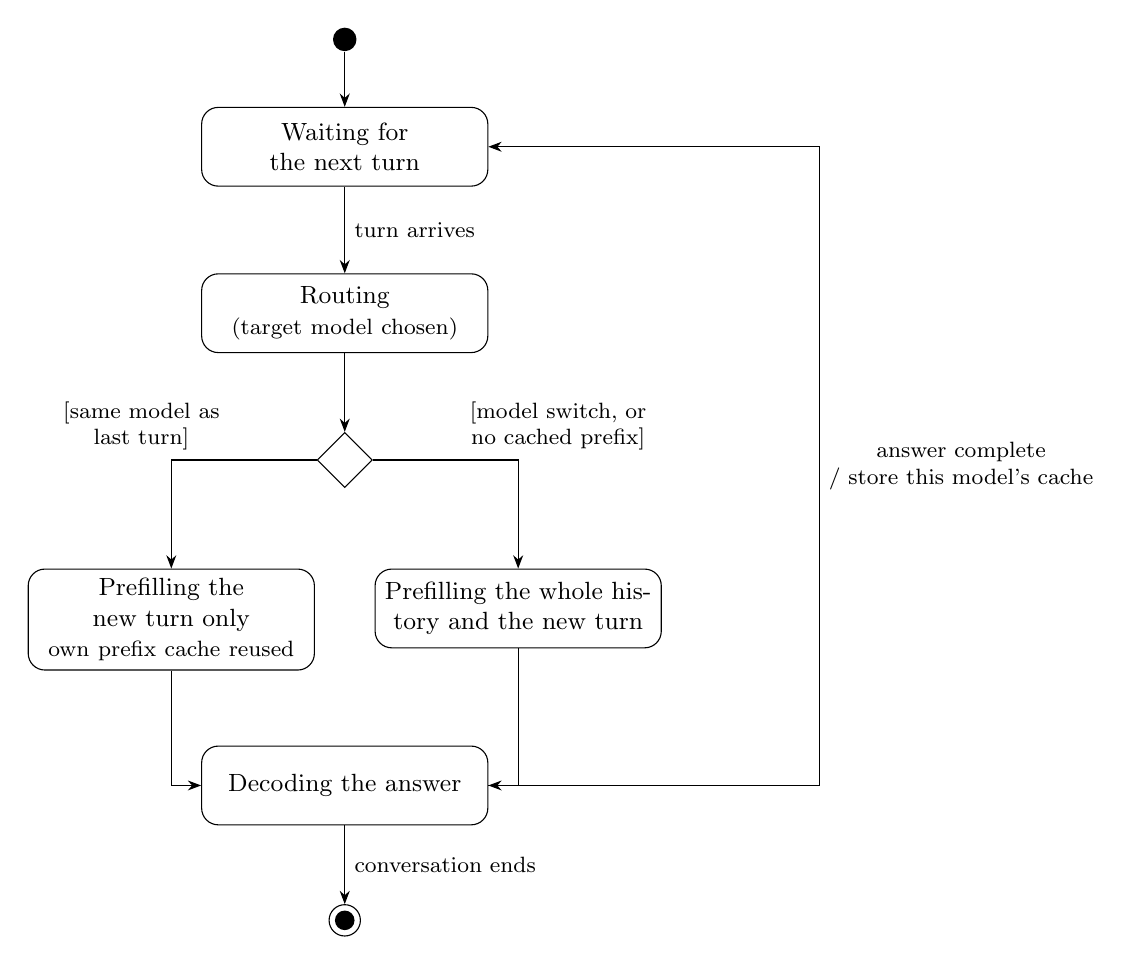
\begin{tikzpicture}[
  >=Stealth, node distance=1.2cm and 1.6cm,
  state/.style={draw, rounded corners=6pt, align=center, minimum height=1.0cm,
    text width=3.4cm, font=\small},
  choice/.style={draw, diamond, aspect=1.4, inner sep=1pt, minimum size=0.7cm},
  lbl/.style={font=\footnotesize, align=center},
  every edge/.style={draw, ->}]
\node[circle, fill, inner sep=3pt] (init) {};
\node[state, below=0.7cm of init] (wait) {Waiting for the next turn};
\node[state, below=1.1cm of wait] (route) {Routing\\\footnotesize(target model chosen)};
\node[choice, below=1.0cm of route] (ch) {};
\node[state, below left=1.2cm and 0.2cm of ch] (hit) {Prefilling the new turn only\\\footnotesize own prefix cache reused};
\node[state, below right=1.2cm and 0.2cm of ch] (full) {Prefilling the whole history and the new turn};
\node[state] (dec) at ($(hit.south)!0.5!(full.south)+(0,-1.6)$) {Decoding the answer};
\node[circle, draw, inner sep=4pt, below=1.0cm of dec] (fin) {};
\node[circle, fill, inner sep=2.5pt] at (fin) {};
\draw[->] (init) -- (wait);
\draw[->] (wait) -- node[lbl, right] {turn arrives} (route);
\draw[->] (route) -- (ch);
\draw[->] (ch) -| node[lbl, above left, pos=0.3] {[same model as\\ last turn]} (hit);
\draw[->] (ch) -| node[lbl, above right, pos=0.3] {[model switch, or\\ no cached prefix]} (full);
\draw[->] (hit) |- (dec);
\draw[->] (full) |- (dec);
\draw[->] (dec.east) -- ++(4.2,0) |- node[lbl, right, pos=0.25] {answer complete\\ / store this model's cache} (wait.east);
\draw[->] (dec) -- node[lbl, right] {conversation ends} (fin);
\end{tikzpicture}}
\caption{Current situation without Tandem (UML state machine for one
conversation turn). After a model switch the new model prefills the whole
history again.}
\label{fig:current-situation}
\end{figure}


\subsection{The Context of the Work}
Figure~\ref{fig:work-context} shows Tandem and the people and systems it
exchanges data with. End users never interact with Tandem directly: they use
an application, which sends each turn to the serving stack. The semantic
router chooses the target model, and the serving engine holds the models and
their KV caches. Operators configure which setups may use prediction and read
the records and error codes; researchers run comparisons and read the reports.
The labels on the arrows are the data exchanged, and match the fields in the
Data Dictionary (Section~\ref{sec:data-dictionary}).

\begin{figure}[H]
\centering
\resizebox{\linewidth}{!}{%
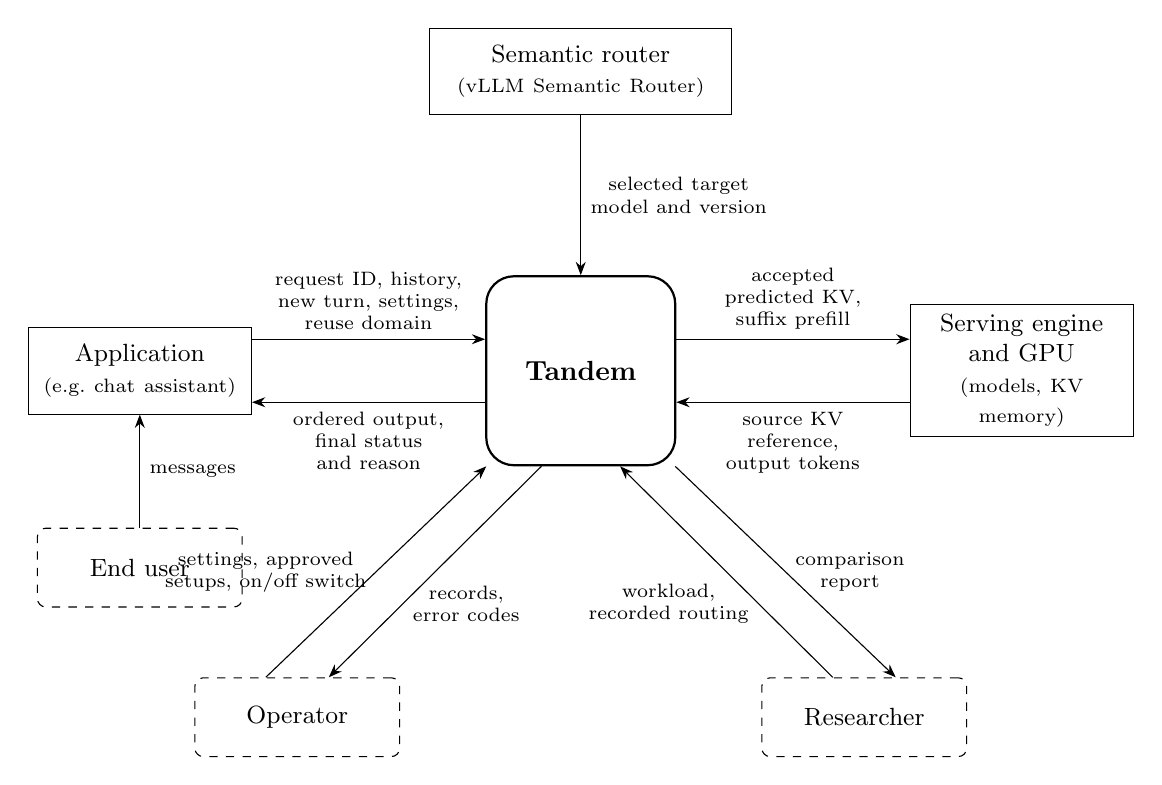
\begin{tikzpicture}[
  >=Stealth,
  sys/.style={draw, thick, rounded corners=10pt, minimum width=2.4cm,
    minimum height=2.4cm, align=center, font=\bfseries},
  ext/.style={draw, text width=2.6cm, minimum height=1.1cm, align=center,
    font=\small},
  person/.style={draw, rounded corners=3pt, dashed, minimum width=2.6cm,
    minimum height=1.0cm, align=center, font=\small},
  lbl/.style={font=\scriptsize, align=center}]
\node[sys] (tandem) at (0,0) {Tandem};
\node[ext] (app) at (-5.6,0) {Application\\\scriptsize(e.g.\ chat assistant)};
\node[person] (user) at (-5.6,-2.5) {End user};
\node[ext, text width=3.6cm] (router) at (0,3.8) {Semantic router\\\scriptsize(vLLM Semantic Router)};
\node[ext] (engine) at (5.6,0) {Serving engine and GPU\\\scriptsize(models, KV memory)};
\node[person] (op) at (-3.6,-4.4) {Operator};
\node[person] (res) at (3.6,-4.4) {Researcher};
\draw[->] (user) -- node[lbl, right] {messages} (app);
\draw[->] ([yshift=4mm]app.east) -- node[lbl, above] {request ID, history,\\ new turn, settings,\\ reuse domain} ([yshift=4mm]tandem.west);
\draw[<-] ([yshift=-4mm]app.east) -- node[lbl, below] {ordered output,\\ final status\\ and reason} ([yshift=-4mm]tandem.west);
\draw[->] (router) -- node[lbl, right] {selected target\\ model and version} (tandem);
\draw[<-] ([yshift=4mm]engine.west) -- node[lbl, above] {accepted\\ predicted KV,\\ suffix prefill} ([yshift=4mm]tandem.east);
\draw[->] ([yshift=-4mm]engine.west) -- node[lbl, below] {source KV\\ reference,\\ output tokens} ([yshift=-4mm]tandem.east);
\draw[->] ([xshift=-4mm]op.north) -- node[lbl, left] {settings, approved\\ setups, on/off switch} ([xshift=-12mm]tandem.south);
\draw[<-] ([xshift=4mm]op.north) -- node[lbl, right, pos=0.35] {records,\\ error codes} ([xshift=-5mm]tandem.south);
\draw[->] ([xshift=-4mm]res.north) -- node[lbl, left, pos=0.35] {workload,\\ recorded routing} ([xshift=5mm]tandem.south);
\draw[<-] ([xshift=4mm]res.north) -- node[lbl, right] {comparison\\ report} ([xshift=12mm]tandem.south);
\end{tikzpicture}}
\caption{Context of the work. Solid boxes are adjacent systems; dashed boxes
are people.}
\label{fig:work-context}
\end{figure}


\subsection{Work Partitioning}
Part I lists external events and exchanged data; Part II summarizes the
corresponding business use cases (BUCs).

\begingroup
\small
\setlength{\tabcolsep}{4pt}
\renewcommand{\arraystretch}{1.18}
\begin{longtable}{|>{\centering\arraybackslash}p{0.14\textwidth}|>{\centering\arraybackslash}p{0.23\textwidth}|>{\centering\arraybackslash}p{0.27\textwidth}|>{\centering\arraybackslash}p{0.27\textwidth}|}
\caption{Work Partitioning Part I}\label{tab:work-partitioning-inputs}\\
\hline
\textbf{Event Number} & \textbf{Event Name} & \textbf{Input} & \textbf{Output}\\
\hline
\endhead
1 & Routed inference request received & Request ID, full prompt, target model selected by vLLM Semantic Router, and generation parameters. & Accepted request with validated inputs, or a rejection with a reason.\\
\hline
2 & Target KV prediction needed after a model switch & Source-model KV tensors or handle, target model, shared-prefix metadata and supported predictor version. & Predicted target-model KV cache and runtime validation result, or native-prefill fallback with a reason.\\
\hline
3 & Response token generated & Generated token, output position and request ID. & Streamed response token associated with the correct request.\\
\hline
4 & Request completed or stopped & Completion, failure, cancellation or timeout event. & Final request status and release of resources no active request still needs.\\
\hline
5 & Benchmark run requested & Held-out conversations, recorded routing decisions, native target KV references, predictor version and serving settings. & Report of KV prediction error, output checks, prediction time, TTFT, throughput, prompt work and GPU time.\\
\hline
6 & Serving configuration changed & Updated model versions, predictor parameters or checkpoints, alignment rules, resource limits or reuse control. & Validated configuration and invalidated incompatible cache references, or a configuration error.\\
\hline
\end{longtable}

\begin{longtable}{|>{\centering\arraybackslash}p{0.14\textwidth}|>{\centering\arraybackslash}p{0.815\textwidth}|}
\caption{Work Partitioning Part II}\label{tab:work-partitioning-bucs}\\
\hline
\textbf{Event Number} & \textbf{Summary of BUC}\\
\hline
\endhead
1 & Validate routed inputs and preserve the target selection; reject invalid requests before generation.\\
\hline
2 & Predict target KV from source KV; validate/load, prefill the suffix and decode, or use native fallback.\\
\hline
3 & Stream ordered tokens under the correct request ID.\\
\hline
4 & Record one final status and release resources without invalidating active shared caches.\\
\hline
5 & Measure held-out KV/output accuracy and matched serving performance, including prediction overhead and cost assumptions.\\
\hline
6 & Apply valid settings, invalidate incompatible caches and disable unqualified setups.\\
\hline
\end{longtable}
\endgroup

\subsection{Specifying a Business Use Case (BUC)}
\textbf{BUC1: Model-switch inference (events 1--4).} Accept the routed request,
predict and validate target KV from source KV, prefill the suffix and decode;
use native fallback when needed. Return ordered output and one final status,
or reject invalid inputs before generation.

\textbf{BUC2: Evaluate a setup (event 5).} Compare held-out KV predictions,
outputs, overhead and serving performance against matched native runs.

\textbf{BUC3: Update serving settings (event 6).} Validate the configuration,
invalidate incompatible caches and keep unqualified setups disabled.


\section{Business Data Model and Data Dictionary}


\subsection{Business Data Model}
A run contains configuration and requests. Each request links its model,
sharing group, source KV, versioned prediction/prefix, output and measurements.
Comparisons pair native/Tandem requests; accepted requests have one final
status, rejections stay separate and applications retain conversation storage.


\subsection{Data Dictionary}
\label{sec:data-dictionary}
These are logical inputs and engine-side state, not an HTTP tensor payload;
retain the full prompt and derive the suffix after prefix validation.
\begin{longtable}{@{}p{0.20\textwidth}p{0.25\textwidth}p{0.49\textwidth}@{}}
\toprule Field & Allowed value & Purpose\\\midrule\endhead
\texttt{run\_id} & Nonempty text & Identifies a test run.\\
\texttt{request\_id} & Nonempty text, unique per run & Links output, final status and measurements.\\
\texttt{history} & Ordered messages & Includes prior conversation and system instructions.\\
\texttt{latest\_message} & Text or role/message & New turn in the target conversation format.\\
\texttt{model\_id} & Known name and exact version & Router-selected target; fixed during replay.\\
\texttt{settings} & Supported generation controls & Output cap, sampling, stops, optional seed; record defaults.\\
\texttt{reuse\_domain} & Host-assigned group ID & Sharing permission; unique per conversation by default, and shared only when the host explicitly enables it. Requests cannot self-authorize.\\
\texttt{source\_kv} & Optional engine cache reference & Source keys/values for the covered prefix.\\
\texttt{predictor} & Versioned supported mapping & Model pair, method, parameters/checkpoint and alignment.\\
\texttt{candidate} & Optional predicted KV reference & Target KV awaiting validation.\\
\texttt{suffix} & Derived target-token sequence & All tokens after the accepted cached prefix.\\
\texttt{cache\_metadata} & Versioned cache description & Source/target/predictor versions, token/layer alignment, prefix/positions, tokenizer/format, precision, sharing group, readiness and configuration version.\\
\texttt{configuration} & Versioned setup & Hardware/software, frozen LLMs, qualified predictors/pairs, limits and reuse switch.\\
\texttt{output\_event} & Request ID, order, token/text & An ordered response fragment.\\
\texttt{status} & Rejected/completed/failed/cancelled & Failures/cancellations may follow partial output.\\
\texttt{reason} & Defined code & Rejection, no reuse, cancellation, timeout or server/resource failure.\\
\texttt{measurement} & Value with units, or missing/reason & Timings, computed/reused tokens and observed memory.\\
\texttt{comparison} & Matched-run results & Speed, throughput, uncertainty, output differences and failures.\\
\bottomrule
\end{longtable}
Input plus requested output must fit model/server limits; the output cap is
positive and unsupported controls are rejected. Unusable optional caches
trigger native processing, while invalid inputs/server failures may prevent
completion. Normal exports omit raw conversations and KV.

\section{The Scope of the Product}


\subsection{Product Boundary}
Tandem includes source-to-target KV predictor development and fitting,
reference-data preparation, engine integration, cache validation/loading,
request isolation, fallback and evaluation on one server. The application
supplies the prompt and settings; vLLM Semantic Router selects the target.
Only supported predictors and exact shared prefixes are reused, and existing
native prefix caching remains enabled in the baseline.

Base-LLM training, router development, document retrieval, agent coordination,
a graphical application and multi-server execution are outside scope.


\subsection{Product Use Case Table}
\begin{longtable}{@{}p{0.12\textwidth}p{0.25\textwidth}p{0.57\textwidth}@{}}
\toprule ID & What happens & Required result\\\midrule\endhead
PUC1 & A model switch has source KV state and a supported predictor & Predict target KV for the shared prefix, load it after runtime checks, prefill the suffix and decode.\\
PUC2 & A cache is missing or fails a check & Process the prompt normally and record why reuse was not used.\\
PUC3 & Reuse fails during processing & Restart safely before output where possible; otherwise report the failure.\\
PUC4 & An operator changes settings & Accept supported settings and reject inconsistent or unsupported ones.\\
PUC5 & An operator or researcher starts a comparison & Run matching requests with and without Tandem and produce a repeatable report.\\
PUC6 & A request is cancelled or times out & Report its final status and release memory no active request needs.\\
\bottomrule
\end{longtable}

\subsection{Individual Product Use Cases (PUC's)}
Figure~\ref{fig:product-use-cases} shows the product use cases from the table
above and the actors that take part in them. The application is the primary
actor for serving a turn (PUC1) and cancelling a request (PUC6); it acts on
behalf of the end user. Serving a turn always includes predicting and checking
the target cache. Native prefill (PUC2) and failure recovery (PUC3) extend it:
they happen only when reuse cannot be used or fails. The router and the
serving engine are secondary actors that PUC1 depends on. The operator changes
settings (PUC4), and the operator or a researcher runs comparisons (PUC5).

\begin{figure}[H]
\centering
\resizebox{\linewidth}{!}{%
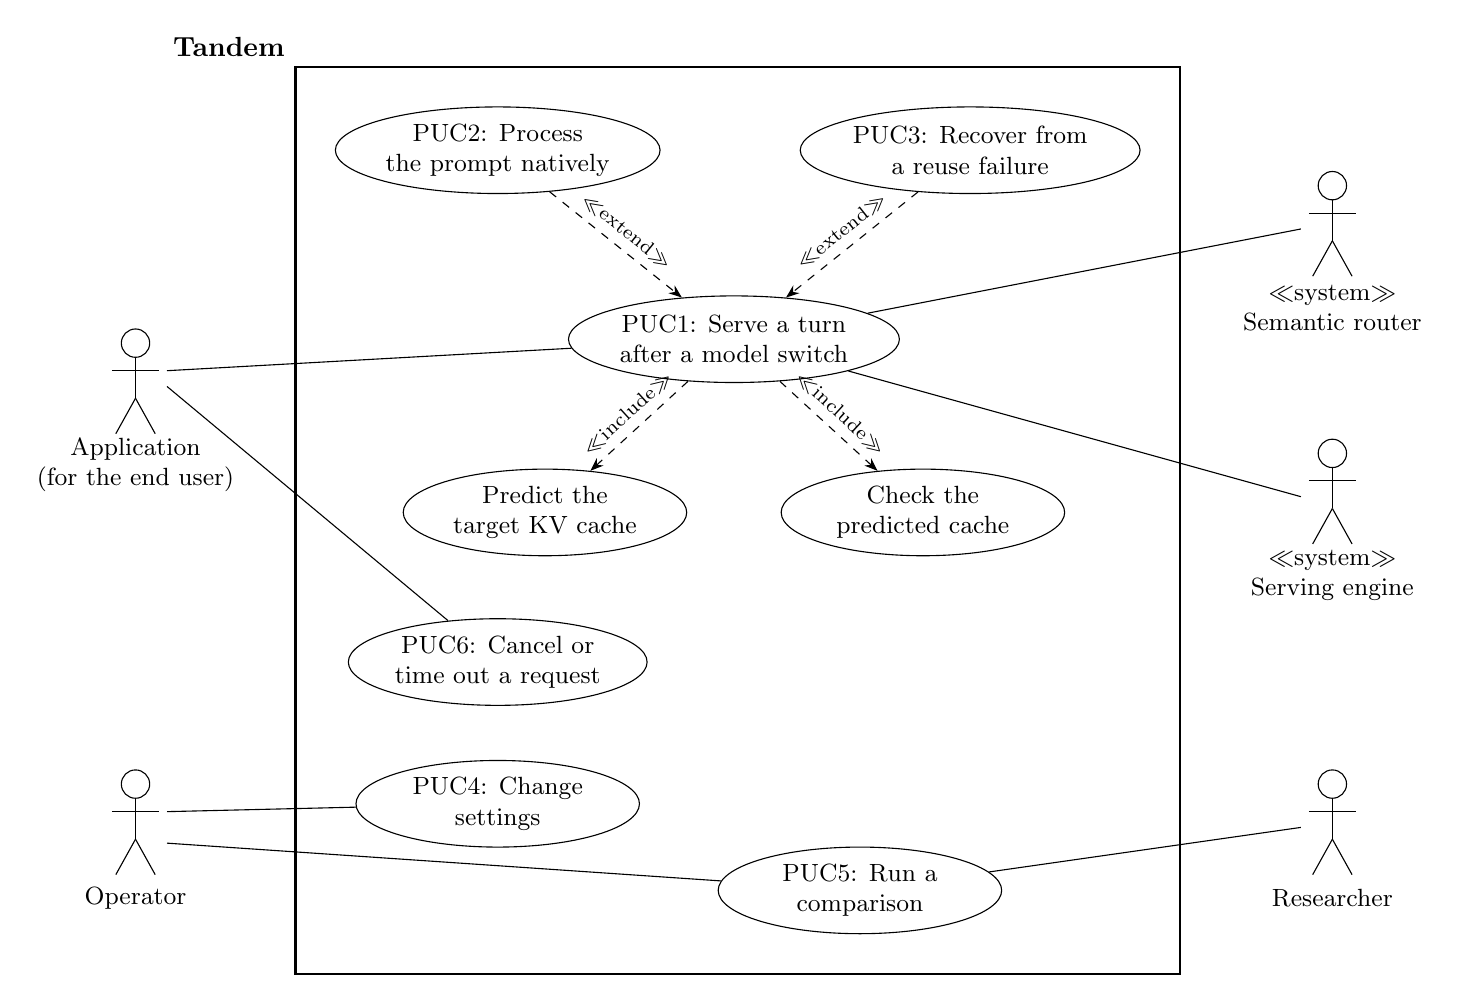
\begin{tikzpicture}[
  >=Stealth,
  uc/.style={draw, ellipse, align=center, font=\small, minimum width=3.6cm,
    minimum height=1.1cm, inner sep=1pt},
  lbl/.style={font=\scriptsize},
  actor/.pic={
    \draw (0,0.55) circle (0.18);
    \draw (0,0.37) -- (0,-0.15);
    \draw (-0.3,0.2) -- (0.3,0.2);
    \draw (0,-0.15) -- (-0.25,-0.6);
    \draw (0,-0.15) -- (0.25,-0.6);}]
\node[uc] (serve) at (0,2.6) {PUC1: Serve a turn\\after a model switch};
\node[uc] (predict) at (-2.4,0.4) {Predict the\\target KV cache};
\node[uc] (check) at (2.4,0.4) {Check the\\predicted cache};
\node[uc] (native) at (-3.0,5.0) {PUC2: Process\\the prompt natively};
\node[uc] (recover) at (3.0,5.0) {PUC3: Recover from\\a reuse failure};
\node[uc] (cancel) at (-3.0,-1.5) {PUC6: Cancel or\\time out a request};
\node[uc] (settings) at (-3.0,-3.3) {PUC4: Change\\settings};
\node[uc] (compare) at (1.6,-4.4) {PUC5: Run a\\comparison};
\node[draw, thick, fit=(serve)(predict)(check)(native)(recover)(cancel)(settings)(compare),
  inner sep=0.5cm, label={[font=\bfseries]north west:Tandem}] (box) {};
\draw[dashed, ->] (serve) -- node[lbl, sloped, above] {$\ll$include$\gg$} (predict);
\draw[dashed, ->] (serve) -- node[lbl, sloped, above] {$\ll$include$\gg$} (check);
\draw[dashed, ->] (native) -- node[lbl, sloped, above] {$\ll$extend$\gg$} (serve);
\draw[dashed, ->] (recover) -- node[lbl, sloped, above] {$\ll$extend$\gg$} (serve);
\pic at (-7.6,2.0) {actor}; \node[font=\small, align=center] (app) at (-7.6,1.0) {Application\\(for the end user)};
\pic at (-7.6,-3.6) {actor}; \node[font=\small] (op) at (-7.6,-4.5) {Operator};
\pic at (7.6,-3.6) {actor}; \node[font=\small] (res) at (7.6,-4.5) {Researcher};
\pic at (7.6,4.0) {actor}; \node[font=\small, align=center] (router) at (7.6,3.0) {$\ll$system$\gg$\\Semantic router};
\pic at (7.6,0.6) {actor}; \node[font=\small, align=center] (engine) at (7.6,-0.4) {$\ll$system$\gg$\\Serving engine};
\draw (-7.2,2.2) -- (serve);
\draw (-7.2,2.0) -- (cancel);
\draw (-7.2,-3.4) -- (settings);
\draw (-7.2,-3.8) -- (compare);
\draw (7.2,-3.6) -- (compare);
\draw (7.2,4.0) -- (serve);
\draw (7.2,0.6) -- (serve);
\end{tikzpicture}}
\caption{Product use cases. Solid lines connect actors to the use cases they
take part in.}
\label{fig:product-use-cases}
\end{figure}


\section{Functional Requirements}


\subsection{Functional Requirements}
\label{sec:functional}
Functional requirements describe what Tandem must do; non-functional
requirements describe its quality and performance. Every requirement in this
document has the same three parts: the requirement (``shall'' means
required), a \emph{fit criterion} that says how to check it, and its
\emph{source and rationale}, which names the goal (G), constraint (C),
business rule (BR) or assumption (A) it comes from and the Hazard Analysis
hazards (H) it mitigates \cite{TandemHA}. Section~\ref{sec:traceability} gives
the full traceability matrix, with each requirement's priority and test.
Detailed test procedures are in the V\&V Plan \cite{TandemVnV}. Named
settings, such as \texttt{LEAK\_CYCLES}, are defined with their values and
reasons in Table~\ref{tab:symbolic-constants}; draft values are reviewed on
development data before final tests (OI3), and are not changed to rescue a
failed final test.

\begin{itemize}
\item \phantomsection\label{req:FR-01}
\textbf{FR-01 --- Check requests before processing}\par
Tandem shall validate each request against the Data Dictionary, and check
request and cache sizes, references and formats against the limits published
under \hyperref[req:NFR-09]{\texttt{NFR-09}}, before allocating any resources
for it.\par
\textbf{Fit criterion.} Requests with missing fields, unknown models, invalid
settings, duplicate IDs or oversized prompts are rejected before generation,
each with a reason code; valid requests without a cache are accepted.
Inconsistent lengths, invalid cache handles and unsupported formats lead to
rejection, native processing or a reported failure, never to repeated
retries.\par
\textbf{Source and rationale.} BR2, A2; H6. An invalid input must be told
apart from a cache miss.

\item \phantomsection\label{req:FR-02}
\textbf{FR-02 --- Use the requested model and inputs}\par
Tandem shall run each request on the router-selected model and revision, with
every message of the prompt in its original order and the accepted generation
settings, without adding, removing or changing any of them.\par
\textbf{Fit criterion.} For each test request, the model ID, revision, prompt
token IDs and generation settings that reach the target model are compared
field by field and token by token with those of native processing of the
same request, and are identical.\par
\textbf{Source and rationale.} BR1, C2, G3; H16. The answer must be the one the
application asked the selected model for.

\item \phantomsection\label{req:FR-03}
\textbf{FR-03 --- Match the shared history exactly}\par
Tandem shall reuse a cache only for an exact prefix of the current history,
as formatted and tokenized for the selected model.\par
\textbf{Fit criterion.} Reuse is blocked when any of the following differs
between the cached prefix and the current history: the text, role or order
of any message; the system instructions; the chat-template version; the
tokenizer version; or a token position. The latest turn is always processed
as new input.\par
\textbf{Source and rationale.} C4; H1. Similar meaning or equal cache sizes do
not make two histories the same.

\item \phantomsection\label{req:FR-04}
\textbf{FR-04 --- Check a predicted cache before reuse}\par
Tandem shall load a predicted cache only if all of these checks pass:
(1) the request is permitted to use it (\hyperref[req:SR-01]{\texttt{SR-01}});
(2) its model pair and predictor version are approved
(\hyperref[req:FR-14]{\texttt{FR-14}}); (3) it covers an exact prefix
(\hyperref[req:FR-03]{\texttt{FR-03}}); (4) its recorded model, tokenizer,
predictor and configuration versions are current
(\hyperref[req:SR-05]{\texttt{SR-05}}); (5) its tensor shapes, layout and
precision match the target model; (6) all its values are finite; (7) its
checksum matches (\hyperref[req:SR-11]{\texttt{SR-11}}); and (8) enough memory
is free without evicting caches in use (\hyperref[req:SR-03]{\texttt{SR-03}}).\par
\textbf{Fit criterion.} Each check is made to fail on its own, and the cache
is rejected each time; a cache that passes all eight is accepted. Missing
information counts as a failed check.\par
\textbf{Source and rationale.} C4, BR6; H1, H3, H9. Any one of these faults
can change the answer without any visible error.

\item \phantomsection\label{req:FR-05}
\textbf{FR-05 --- Load the predicted cache and prefill the rest of the prompt}\par
Tandem shall load an accepted predicted cache, prefill the tokens after the
cached prefix once each and in order, and decode with the selected target
model.\par
\textbf{Fit criterion.} The cached prefix length plus the number of prefilled
tokens equals the native prompt length; the prefilled token IDs and positions
equal those of native processing after the prefix; and the output passes
\hyperref[req:NFR-05]{\texttt{NFR-05}} for same-model reuse or
\hyperref[req:SR-09]{\texttt{SR-09}} for cross-model reuse.\par
\textbf{Source and rationale.} G1; H16. This is where the saved prefill work
comes from.

\item \phantomsection\label{req:FR-06}
\textbf{FR-06 --- Keep native processing available}\par
Tandem shall process a request natively, with the engine's own prefix
caching, whenever prediction is switched off, no predicted cache is
available, or any check in \hyperref[req:FR-04]{\texttt{FR-04}} fails.\par
\textbf{Fit criterion.} Same-model turns, unshared histories, missing caches
and unapproved model pairs are each processed natively, with a recorded
reason, and their output equals the native reference.\par
\textbf{Source and rationale.} C5, BR2; H1, H6. A cache miss must never cause
a valid request to fail.

\item \phantomsection\label{req:FR-07}
\textbf{FR-07 --- Answer or report after a prediction or reuse failure}\par
If prediction, checking or cache loading fails before any output token has
been returned, Tandem shall answer the request by native processing under the
same request ID. If native processing then also fails, or if any failure
happens after output has started, Tandem shall end the request with status
\texttt{failed} and a reason. A response shall never contain output from two
attempts.\par
\textbf{Fit criterion.} Predictor exceptions, invalid tensors and loading
failures injected before output each end in a natively produced answer under
the original request ID, with no repeated output. Failures injected after
output has started, or during the native answer, end with status
\texttt{failed}. No request is attempted more than twice.\par
\textbf{Source and rationale.} C5; H7. Prevents retry loops and answers mixed
from two attempts.

\item \phantomsection\label{req:FR-08}
\textbf{FR-08 --- Keep output attached to the right request}\par
Tandem shall return each request's output in order under its own request ID,
and record exactly one final status for each accepted request.\par
\textbf{Fit criterion.} Under overlapping requests, cancellations and
failures, every output event carries the right request ID in order, and each
accepted request ends with exactly one of \texttt{completed}, \texttt{failed}
or \texttt{cancelled}; rejected requests have a separate rejection record.\par
\textbf{Source and rationale.} BR4; H2. Prevents one user receiving another's
answer, and duplicate answers.

\item \phantomsection\label{req:FR-09}
\textbf{FR-09 --- Release memory when a request ends}\par
When a request ends, Tandem shall release every allocation that belongs only
to that request. Caches still used by an active request, the engine's prefix
cache, and predicted caches kept under \hyperref[req:SR-14]{\texttt{SR-14}}
are kept.\par
\textbf{Fit criterion.} After \texttt{LEAK\_CYCLES} cycles of completion,
failure and cancellation, no ended request owns an allocation, outputs of
active requests are unchanged, and kept caches stay within the
\hyperref[req:SR-14]{\texttt{SR-14}} limit.\par
\textbf{Source and rationale.} G2; H4, H6. Prevents memory leaks without
discarding caches that later turns can reuse.

\item \phantomsection\label{req:FR-10}
\textbf{FR-10 --- Record what happened for each request}\par
Tandem shall record, for each request, the run and request IDs, the source and
target models, the predictor version, timings, the number of prompt tokens
computed and reused, which reused positions were predicted, the final status,
and the reuse decision with its reason, in a structured format.\par
\textbf{Fit criterion.} For a known prompt, every field is present and the
token counts equal the known values; a measurement that is unavailable is
recorded as missing with a reason, never estimated.\par
\textbf{Source and rationale.} BR4, BR5; H11, H17. Saved work and failures
must be visible to be checked.

\item \phantomsection\label{req:FR-11}
\textbf{FR-11 --- Compare against a matched native run}\par
Tandem shall provide a comparison mode that runs the same requests, recorded
routing decisions, arrival times and generation settings once with Tandem and
once natively, with the engine's prefix caching on in both runs.\par
\textbf{Fit criterion.} The two runs' configuration and request records are
identical apart from the prediction switch; any other difference marks the
comparison invalid in its report.\par
\textbf{Source and rationale.} BR5; H11. A speedup is only meaningful against
the same work done natively.

\item \phantomsection\label{req:FR-12}
\textbf{FR-12 --- Make comparison results repeatable}\par
Tandem's comparison mode shall report, for each request and for the whole run,
KV prediction error, prediction and response times, throughput, prompt work,
total GPU time, GPU time per completed request, output differences and
fallback outcomes, together with the versions, hardware, data split, seeds
and repetitions used.\par
\textbf{Fit criterion.} Rerunning a report's recorded configuration on the
same hardware reproduces its token counts exactly and its timings within
their confidence intervals. Prediction, checking and loading time are
included in the totals; offline training cost is reported separately.\par
\textbf{Source and rationale.} BR5, G2; H11. Results must be reproducible to
be trusted.

\item \phantomsection\label{req:FR-13}
\textbf{FR-13 --- Control which setups may use prediction}\par
Tandem shall provide a switch that turns prediction on and off, keep a record
of approved model pairs, predictor versions and checkpoints, and reject a
configuration that names an unapproved setup or sets a limit outside the
range published under \hyperref[req:NFR-09]{\texttt{NFR-09}}.\par
\textbf{Fit criterion.} Inconsistent or out-of-range settings are rejected
with a reason; unapproved combinations are processed natively; caches made
under a previous configuration are invalidated after a change.\par
\textbf{Source and rationale.} BR6; H3, H13. Loading a model is not evidence
that prediction for it is safe.

\item \phantomsection\label{req:FR-14}
\textbf{FR-14 --- Test a setup before enabling prediction}\par
Tandem shall enable prediction for a setup only when its approval record shows
a pass for each of: output quality (\hyperref[req:NFR-05]{\texttt{NFR-05}} for
same-model reuse, \hyperref[req:SR-09]{\texttt{SR-09}} for cross-model
reuse); privacy (\hyperref[req:SR-01]{\texttt{SR-01}},
\hyperref[req:SR-04]{\texttt{SR-04}} and \hyperref[req:SR-06]{\texttt{SR-06}});
and failure handling (\hyperref[req:FR-07]{\texttt{FR-07}} and
\hyperref[req:SR-02]{\texttt{SR-02}}). The record also lists the predictor
and data versions, the data split and the measured KV error.\par
\textbf{Fit criterion.} Removing any one test result from the record, or
replacing it with a failure, keeps prediction disabled for that setup. The
fitting and test data share no conversations.\par
\textbf{Source and rationale.} BR6; H8, H11. Quality must be shown before
any speed claim.

\item \phantomsection\label{req:FR-15}
\textbf{FR-15 --- Stop cancelled or timed-out requests}\par
Tandem shall let the application cancel a request, and shall end any request
that runs longer than its timeout (\texttt{DEFAULT\_TIMEOUT} unless the
deployment sets another).\par
\textbf{Fit criterion.} A request cancelled while queued or running, or one
that exceeds its timeout, returns no output after the cancellation or timeout
is processed, ends with status \texttt{cancelled} and the matching reason, and
has its resources released under \hyperref[req:FR-09]{\texttt{FR-09}}; other
requests' outputs are unchanged.\par
\textbf{Source and rationale.} G4; H6. A request that never ends holds GPU
memory and delays others.

\item \phantomsection\label{req:FR-16}
\textbf{FR-16 --- Predict the target model's KV cache from the source model's}\par
Tandem shall predict the target model's keys and values for the shared
history from the source model's KV cache and the recorded token and layer
alignment, using an approved model pair and predictor version. The target
model shall not prefill the shared history to build the prediction; the only
target-model computation over the history is the run-time check in
\hyperref[req:SR-10]{\texttt{SR-10}}, which recomputes at most
\texttt{CANARY\_TOKENS} of its final tokens.\par
\textbf{Fit criterion.} On held-out conversations, the predicted cache has the
target model's layout, its KV error per layer is reported against offline
native references, the request record shows no target prefill over the
history apart from the \hyperref[req:SR-10]{\texttt{SR-10}} tokens, and
loading and output pass \hyperref[req:FR-05]{\texttt{FR-05}}. The predictor's
architecture, parameters and training procedure are recorded.\par
\textbf{Source and rationale.} G1, C3; H1, H8, H13, H15. Predicting the cache
is Tandem's core function.

\item \phantomsection\label{req:FR-17}
\textbf{FR-17 --- Predict only when the history is long enough to gain}\par
Tandem shall use prediction only when the shared history is at least
\texttt{MIN\_REUSE\_TOKENS} target tokens long for the approved setup, and
process shorter histories natively.\par
\textbf{Fit criterion.} A history shorter than \texttt{MIN\_REUSE\_TOKENS} is
processed natively with reason \texttt{below\_min\_length}. In the TTFT
benchmark, at every tested history length of at least
\texttt{MIN\_REUSE\_TOKENS}, the upper confidence bound of the predicted arm's
median TTFT is no higher than the native median.\par
\textbf{Source and rationale.} G2, G4; H15. For short histories, prediction,
checking and loading can cost more than native prefill.
\end{itemize}

\par\medskip\noindent\phantomsection\label{sec:formal}
\textbf{KV prediction and reuse rules.}
Tandem's core operation is:
\[
 \widehat{\mathrm{KV}}_{\mathrm{target}}
 = f_\theta(\mathrm{KV}_{\mathrm{source}}).
\]
The left side is the predicted target cache. The function $f_\theta$ is the
predictor, with versioned parameters $\theta$, for an approved source and
target model pair and a recorded token and layer alignment. Base LLM weights
stay frozen.

For a request $r$ with selected model $m_r$, history $h_r$ and reuse domain
$d_r$, and a predicted cache $c$ built for model $m_c$ from history $h_c$ in
domain $d_c$, prediction is used exactly when the predicate $\mathit{reuse}(r,
c)$ holds:
{\small
\begin{align*}
\mathit{reuse}(r, c) \iff{} & \mathit{enabled} \wedge
  \mathit{approved}(m_{\mathrm{source}}, m_r, \theta)
  && \text{FR-13, FR-14}\\
 {}\wedge{} & m_c = m_r \wedge d_c = d_r
  && \text{FR-02, SR-01}\\
 {}\wedge{} & h_c \text{ is a prefix of } h_r \wedge
  \lvert h_c\rvert \ge \texttt{MIN\_REUSE\_TOKENS}
  && \text{FR-03, FR-17}\\
 {}\wedge{} & \mathit{checks}(c) \wedge
  \mathit{err}_{\mathrm{canary}}(c) \le \texttt{CANARY\_LIMIT}
  && \text{FR-04, SR-10}
\end{align*}}
Here $\mathit{checks}(c)$ is the conjunction of the eight checks in
\hyperref[req:FR-04]{\texttt{FR-04}}, and $\mathit{err}_{\mathrm{canary}}(c)$
is the largest relative error between the predicted and recomputed keys and
values over the last \texttt{CANARY\_TOKENS} history positions
(\hyperref[req:SR-10]{\texttt{SR-10}}). For a tensor $X$ and its reference
$X^\ast$, the relative error is $\lVert X - X^\ast\rVert_F /
\lVert X^\ast\rVert_F$. Let $P(c)$ be the set of positions in $c$ whose keys
and values were predicted rather than computed by the target model
(\hyperref[req:SR-15]{\texttt{SR-15}}). Then a cache used as the source of a
new prediction must have $P = \emptyset$.

The outcome of a valid request then follows Table~\ref{tab:outcome}, where
\emph{fails early} means a failure before any output token is returned.

\begin{table}[H]
\centering
\small
\caption{Outcome of a valid request}
\label{tab:outcome}
\begin{tabular}{@{}cccp{0.45\textwidth}@{}}
\toprule
$\mathit{reuse}(r,c)$ & Fails early & Fails after output & Outcome\\
\midrule
true & no & no & Load $c$, prefill the suffix, decode: \texttt{completed}\\
true & yes & -- & Native processing, same request ID (FR-07)\\
false & -- & no & Native processing (FR-06)\\
either & -- & yes & \texttt{failed}; no second attempt (FR-07)\\
\bottomrule
\end{tabular}
\end{table}

A request that is cancelled or times out at any point ends
\texttt{cancelled} (FR-15). Figure~\ref{fig:tandem-states} shows the same
rules as a UML state machine for one request.

\begin{figure}[H]
\centering
\resizebox{\linewidth}{!}{%
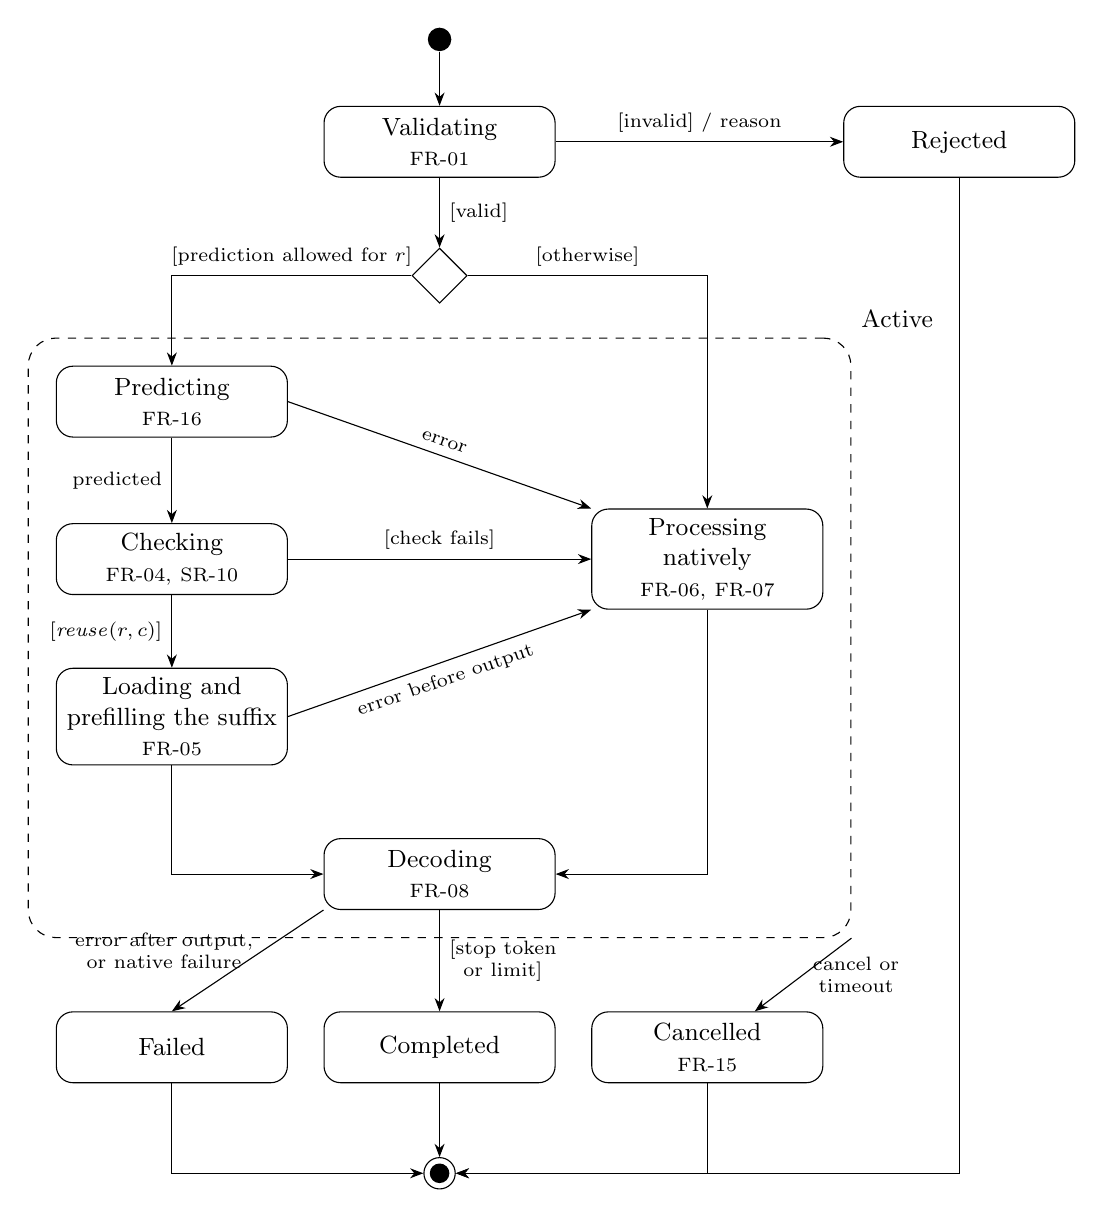
\begin{tikzpicture}[
  >=Stealth,
  state/.style={draw, rounded corners=6pt, align=center, minimum height=0.9cm,
    text width=2.7cm, font=\small},
  choice/.style={draw, diamond, aspect=1.4, inner sep=1pt, minimum size=0.7cm},
  lbl/.style={font=\scriptsize, align=center}]
\node[circle, fill, inner sep=3pt] (init) at (0,0) {};
\node[state] (validate) at (0,-1.3) {Validating\\\scriptsize FR-01};
\node[choice] (ch) at (0,-3.0) {};
\node[state] (predict) at (-3.4,-4.6) {Predicting\\\scriptsize FR-16};
\node[state] (check) at (-3.4,-6.6) {Checking\\\scriptsize FR-04, SR-10};
\node[state] (load) at (-3.4,-8.6) {Loading and prefilling the suffix\\\scriptsize FR-05};
\node[state] (native) at (3.4,-6.6) {Processing natively\\\scriptsize FR-06, FR-07};
\node[state] (decode) at (0,-10.6) {Decoding\\\scriptsize FR-08};
\node[draw, dashed, rounded corners=10pt, inner sep=0.35cm,
  fit=(predict)(check)(load)(native)(decode),
  label={[font=\small]north east:Active}] (active) {};
\node[state] (rejected) at (6.6,-1.3) {Rejected};
\node[state] (completed) at (0,-12.8) {Completed};
\node[state] (failed) at (-3.4,-12.8) {Failed};
\node[state] (cancelled) at (3.4,-12.8) {Cancelled\\\scriptsize FR-15};
\node[circle, draw, inner sep=4pt] (fin) at (0,-14.4) {};
\node[circle, fill, inner sep=2.5pt] at (fin) {};
\draw[->] (init) -- (validate);
\draw[->] (validate) -- node[lbl, above] {[invalid] / reason} (rejected);
\draw[->] (validate) -- node[lbl, right] {[valid]} (ch);
\draw[->] (ch) -| node[lbl, above, pos=0.25] {[prediction allowed for $r$]} (predict);
\draw[->] (ch) -| node[lbl, above, pos=0.25] {[otherwise]} (native);
\draw[->] (predict) -- node[lbl, left] {predicted} (check);
\draw[->] (check) -- node[lbl, left] {[$\mathit{reuse}(r,c)$]} (load);
\draw[->] (predict.east) -- node[lbl, above, sloped] {error} (native.north west);
\draw[->] (check) -- node[lbl, above] {[check fails]} (native);
\draw[->] (load.east) -- node[lbl, below, sloped] {error before output} (native.south west);
\draw[->] (load) |- (decode);
\draw[->] (native) |- (decode);
\draw[->] (decode) -- node[lbl, right] {[stop token\\ or limit]} (completed);
\draw[->] (decode.south west) -- node[lbl, left, pos=0.4] {error after output,\\ or native failure} (failed.north);
\draw[->] (active.south east) -- node[lbl, right] {cancel or\\ timeout} (cancelled);
\draw[->] (completed) -- (fin);
\draw[->] (failed) |- (fin);
\draw[->] (cancelled) |- (fin);
\draw[->] (rejected) |- (fin);
\end{tikzpicture}}
\caption{Tandem's handling of one request (UML state machine). Every
transition out of the Active composite state on cancellation or timeout leads
to Cancelled. Each final state records one final status.}
\label{fig:tandem-states}
\end{figure}

\textbf{Accuracy checks.}
\begin{itemize}
\item Native target KV is computed offline as the reference for the same
history. For each layer, report the absolute prediction error as a Frobenius
norm, and the relative error as that norm divided by the reference norm,
separately for keys and values. If the reference norm is zero, report the
absolute error and mark the relative error undefined. A small KV error alone
does not show that outputs are acceptable.
\item \textbf{Same-model reuse} (a cache computed by the target model itself)
must be exact up to numerical noise: corresponding logits (next-token scores)
after identical earlier tokens may differ by at most \texttt{SCORE\_ATOL} plus
\texttt{SCORE\_RTOL} times the absolute native score, and greedy decoding must
return identical tokens for \texttt{GREEDY\_TOKENS} tokens or until both runs
stop earlier (\hyperref[req:NFR-05]{\texttt{NFR-05}}). Native-run
repeatability is checked first. Unexpected nonfinite values fail.
\item \textbf{Cross-model reuse} (a predicted cache) is approximate, so it
cannot meet those exact limits. It must instead keep the task score within
\texttt{QUALITY\_LOSS\_LIMIT} of native prefill on a held-out test set
(\hyperref[req:SR-09]{\texttt{SR-09}}); logit and token agreement are reported
as diagnostics.
\item Sampling settings need their own recorded qualification, or are
processed natively; equal seeds alone do not guarantee matching outputs.
These checks apply to the declared test set and settings, not to every
possible prompt.
\end{itemize}

Final tests use paired source and native-target KV caches for held-out
conversations, with no fitting or threshold tuning on final results. They
cover the declared limits, same-model and model-switch requests, shared and
unshared histories, cold and warm caches, accepted, missing and rejected
predictions, concurrency and forced failures. Prompts, routing, settings,
arrival times and resource limits are matched, and cache preparation and hits
are recorded.

Timing starts with \texttt{WARMUP\_RUNS} untimed warm-up runs and
\texttt{TIMED\_PAIRS} alternating timed pairs, adding pairs if the uncertainty
is too large. Reports include skips, failures, uncertainty, slowdowns and
negative results. Throughput counts successful completions from the first
arrival to the last final status. TTFT is missing if no token is returned;
end-to-end time, prompt work and directly measured memory are reported
separately.

\section{Look and Feel Requirements}


\subsection{Appearance Requirements}
\textbf{Not Applicable.}


\subsection{Style Requirements}
\begin{itemize}
\item \phantomsection\label{req:NFR-11}
\textbf{NFR-11 --- Report outcomes in plain text}\par
Tandem's records, reports and messages shall use the terms in the glossary
and the defined status and reason codes, and shall not rely on colour or
layout to carry meaning. Tandem shall not restyle or rewrite generated
responses.\par
\textbf{Fit criterion.} Every status and reason code in a sample report
appears in the release's code list (\hyperref[req:NFR-12]{\texttt{NFR-12}});
the report reads the same when printed in black and white; generated output
equals the model's output byte for byte.\par
\textbf{Source and rationale.} BR4. Operators read results in terminals and
scripts parse them.
\end{itemize}


\section{Usability and Humanity Requirements}


\subsection{Ease of Use Requirements}
Ordinary requests use the existing serving interface; only technical users configure KV prediction.

\begin{itemize}
\item \phantomsection\label{req:NFR-02}
\textbf{NFR-02 --- Make setup instructions usable}\par
A technical user with the listed prerequisites shall be able to install Tandem and run the basic example by following its instructions.\par
\textbf{Fit criterion.} An independent reviewer who has not used Tandem follows every documented command in a clean supported environment and gets the documented results without help.\par
\textbf{Source and rationale.} Hands-on users (Section~2.4), DR-01. Operators need a repeatable setup.
\end{itemize}

\subsection{Personalization and Internationalization Requirements}
\textbf{Not Applicable.}


\subsection{Learning Requirements}
Provide a supported installation example explaining KV prediction, fallback
and results under \hyperref[req:DR-01]{\texttt{DR-01}} and
\hyperref[req:NFR-02]{\texttt{NFR-02}}.


\subsection{Understandability and Politeness Requirements}
Messages identify outcomes, invalid fields and corrective actions without exposing private prompts or cache data.

\begin{itemize}
\item \phantomsection\label{req:NFR-01}
\textbf{NFR-01 --- Make results readable}\par
Tandem shall provide readable results with clear field names and units, plus structured data that other programs can read.\par
\textbf{Fit criterion.} From a report alone, without engine internals, a reader can tell for each request whether it used reuse, native processing, fallback after a failed check, or failed.\par
\textbf{Source and rationale.} BR4. Developers and operators need results they can act on.
\end{itemize}


\subsection{Accessibility Requirements}
Commands, reports and instructions use readable text, require no particular
visual editor, and provide machine-readable results without colour-dependent meanings.


\section{Performance Requirements}


\subsection{Speed and Latency Requirements}
\label{sec:performance}
Measure TTFT, end-to-end latency and throughput on preselected workloads,
including non-reuse cases. Timing includes queueing, source retrieval,
prediction, checks/loading, suffix prefill and decoding; handle model loading
consistently. Separate predictor/loading/engine timings and offline development
costs, and retain failures and cancellations.

Compare median TTFT, p95 TTFT (the 95th-percentile wait) and successful
requests per second against the native engine. Estimate confidence
intervals at the draft \texttt{CONFIDENCE\_LEVEL} using
\texttt{BOOTSTRAP\_RESAMPLES} bootstrap resamples
of complete paired trials; record the random seed. Requests within one trial are not independent
repetitions. Use the conservative interval bounds to decide whether an
improvement or allowed slowdown has been demonstrated.

\begin{itemize}
\item \phantomsection\label{req:NFR-04}
\textbf{NFR-04 --- Show a useful reduction in waiting time}\par
On at least one preselected model-switch workload, Tandem shall reduce computed prompt work and median TTFT beyond timing variation.\par
\textbf{Fit criterion.} On that workload, fewer prompt tokens are computed, the upper confidence bound of Tandem's median TTFT is below the lower bound of the native median, output passes \hyperref[req:SR-09]{\texttt{SR-09}}, and there are no additional failures. All workloads are reported, including slowdowns.\par
\textbf{Source and rationale.} G3, G4; H15. This is the measured benefit the project sets out to show.
\end{itemize}

\subsection{Safety-Critical Requirements}
\textbf{Not Applicable.}


\subsection{Precision or Accuracy Requirements}
Evaluate KV error and outputs separately. Review strict draft tolerances on
development data/native variation before final tests (OI3); runtime validation
cannot prove accuracy, and output consistency does not prove factual correctness.

\begin{itemize}
\item \phantomsection\label{req:NFR-05}
\textbf{NFR-05 --- Same-model reuse gives the same output}\par
When a request reuses a cache computed by the target model itself, its output shall match native processing within the limits in the accuracy checks. Cross-model reuse is approximate and is covered by \hyperref[req:SR-09]{\texttt{SR-09}} instead.\par
\textbf{Fit criterion.} On the declared test set, every logit is within \texttt{SCORE\_ATOL} plus \texttt{SCORE\_RTOL} times the absolute native score, and greedy output is identical for \texttt{GREEDY\_TOKENS} tokens or until an earlier shared stop. A mismatch prevents approval; limits are not changed after a failed final test.\par
\textbf{Source and rationale.} BR6; H1, H17. Reusing a model's own cache must not change its answer.


\item \phantomsection\label{req:NFR-03}
\textbf{NFR-03 --- Preserve supported text}\par
Tandem shall preserve valid Unicode text through the selected model's normal conversation formatting and tokenization.\par
\textbf{Fit criterion.} For prompts with accents, non-Latin scripts, unusual whitespace and template delimiters, the prompt token IDs equal those of native processing.\par
\textbf{Source and rationale.} C4, A7; H1. A change in the text would cause false prefix matches or misses.
\end{itemize}


\subsection{Robustness or Fault-Tolerance Requirements}
A failed optional prediction uses native processing when possible; unavailable models or exhausted resources produce an explicit failure.

\begin{itemize}
\item \phantomsection\label{req:NFR-06}
\textbf{NFR-06 --- Report failures and allow later normal requests}\par
Tandem shall explain failures and retain native processing after recoverable cache errors.\par
\textbf{Fit criterion.} After injected incomplete or mismatched caches, allocation failures and timeouts, each handled under \hyperref[req:FR-07]{\texttt{FR-07}}, the next valid request completes natively while the engine is healthy; an unrecoverable engine is reported with a code that asks for operator action.\par
\textbf{Source and rationale.} C5, BR2; H6. One bad cache must not take the service down.

\item \phantomsection\label{req:SR-13}
\textbf{SR-13 --- Limit the load from fallbacks}\par
Tandem shall admit fallback prefills only within the engine's configured
prefill budget, queue at most \texttt{QUEUE\_LIMIT} further requests, and
reject any beyond that with a status telling the caller to retry, instead of
letting them time out. It shall turn cross-model prediction off automatically,
and report this to the operator, when more than
\texttt{FALLBACK\_RATE\_LIMIT} of the last \texttt{FALLBACK\_WINDOW}
predictions fell back.\par
\textbf{Fit criterion.} A test invalidates all caches at once under load:
admitted requests stay within \texttt{REGRESSION\_LIMIT} of the same load
without Tandem (\hyperref[req:NFR-08]{\texttt{NFR-08}}), excess requests get the
retry status instead of timing out, and prediction is turned off.\par
\textbf{Source and rationale.} BR2; H14. Many fallbacks at once must not
overload the server.
\end{itemize}

\subsection{Capacity Requirements}
Publish and test the supported prompt lengths, concurrency and memory limits for each model/hardware setup.

\begin{itemize}
\item \phantomsection\label{req:NFR-07}
\textbf{NFR-07 --- Handle more requests without excessive delay}\par
On at least one preselected shared-history workload, Tandem shall improve throughput within the permitted p95 TTFT increase.\par
\textbf{Fit criterion.} Confidence intervals show higher throughput, and a p95 TTFT increase of at most \texttt{REGRESSION\_LIMIT} times the native value, with no extra failures. Requests and arrival times are recorded.\par
\textbf{Source and rationale.} G4; H14. A capacity gain is only useful if delays stay acceptable.

\item \phantomsection\label{req:SR-14}
\textbf{SR-14 --- Bound the memory held by predicted caches}\par
Memory held by predicted caches that no active request uses shall not exceed
\texttt{PREDICTED\_CACHE\_LIMIT}, and each such cache shall be released after
\texttt{PREDICTED\_CACHE\_TTL} without use.\par
\textbf{Fit criterion.} A test predicts caches that are never used; memory
held by them never exceeds the limit, and each is released within the TTL.\par
\textbf{Source and rationale.} G2; H12. Predictions for turns that never come
must not crowd out active requests.


\item \phantomsection\label{req:NFR-08}
\textbf{NFR-08 --- Limit slowdowns for normal requests}\par
For requests that do not use prediction, Tandem shall keep latency increases and throughput losses within the allowed limit.\par
\textbf{Fit criterion.} Using the conservative confidence-interval bounds, median and p95 TTFT increase by at most \texttt{REGRESSION\_LIMIT} times their native values, and throughput falls by at most the same fraction. A result with too much uncertainty is reported as inconclusive.\par
\textbf{Source and rationale.} G4, BR2; H15. Requests that gain nothing from Tandem must not pay much for it.
\end{itemize}

\subsection{Scalability or Extensibility Requirements}
The initial scope is one server and tested model pairs; extra GPUs, model families, conversation branches and multi-server scaling require further qualification or expanded scope.

\begin{itemize}
\item \phantomsection\label{req:NFR-09}
\textbf{NFR-09 --- Publish supported models and limits}\par
Each release shall list tested setups, limits on simultaneous requests and tokens, and unsupported settings.\par
\textbf{Fit criterion.} Each published limit is tested at its boundary and just beyond it; every setup listed as supported has a passing test record, and untested setups are listed as experimental or disabled.\par
\textbf{Source and rationale.} BR6; H6. Users must be able to tell tested support from untested.
\end{itemize}

\subsection{Longevity Requirements}
Maintain the prototype through the final capstone release, retain versioned
code/test records, and qualify model or dependency updates before claiming support.


\section{Operational and Environmental Requirements}


\subsection{Expected Physical Environment}
\textbf{Not Applicable.}


\subsection{Wider Environment Requirements}
GPU results require the recorded Linux/model/software setup; local CPU checks do not establish serving performance.

\begin{itemize}
\item \phantomsection\label{req:NFR-10}
\textbf{NFR-10 --- Record how to recreate the test setup}\par
Each tested release shall record the hardware, software and commands needed to recreate the setup on compatible hardware.\par
\textbf{Fit criterion.} A team member rebuilds the setup from the record alone, and the basic and output tests pass; the record names the model, dependency and build versions, and any hardware or competing-load difference is reported with repeated timings.\par
\textbf{Source and rationale.} BR5, A6; H11. The setup affects both timing and output.
\end{itemize}

\subsection{Requirements for Interfacing with Adjacent Systems}
Use the existing serving interface, router-selected target model and
engine-managed source KV reference; load validated predicted target KV through
the engine integration. The Data Dictionary defines these fields, and the
application assigns user identity and reuse domains. It gives each conversation
its own domain unless the host explicitly enables sharing.


\subsection{Productization Requirements}
\textbf{Not Applicable.}


\subsection{Release Requirements}
Publish versioned code, dependencies, supported setups, limits and test
results; failed or untested combinations remain experimental or disabled.


\section{Maintainability and Support Requirements}


\subsection{Maintenance Requirements}
\textbf{Not Applicable.}


\subsection{Supportability Requirements}
Use repository issues with version details, error codes and non-private reproduction steps; no support response time is promised.

\begin{itemize}
\item \phantomsection\label{req:NFR-12}
\textbf{NFR-12 --- Explain status and error codes}\par
The release shall explain rejection, fallback and failure codes, including what the operator should do or whether no action is needed.\par
\textbf{Fit criterion.} Each code is triggered in a test and the observed outcome matches its documentation; diagnostics identify the setup for reproduction while meeting \hyperref[req:SR-06]{\texttt{SR-06}}.\par
\textbf{Source and rationale.} BR4. Operators must tell an unused cache from a failed request.
\end{itemize}

\subsection{Adaptability Requirements}
\textbf{Not Applicable.}


\section{Security Requirements}

\subsection{Access Requirements}
\label{sec:security}
\textbf{Not Applicable.}

\subsection{Integrity Requirements}
Use only complete, current, checked caches, and protect state needed by
active requests. SR-07 and SR-08 were merged into FR-01 and FR-07 in version
0.5, so their numbers are not used. SR-09 to SR-15 come from the Hazard
Analysis \cite{TandemHA}.

\par\medskip\noindent\phantomsection\label{req:SR-02}
\textbf{SR-02 --- Do not use incomplete or incompatible caches}\par
Tandem shall reject incomplete, inconsistent, outdated, unsupported or unqualified caches.\par
\textbf{Fit criterion.} Vary each condition; rejected caches never enter generation. Use native processing or report server/resource failure; missing evidence means unsupported.\par
\textbf{Source and rationale.} C4, BR6; H1, H3. Prevents use of an invalid cache.

\par\medskip\noindent\phantomsection\label{req:SR-09}
\textbf{SR-09 --- Limit the quality loss of each cross-model setup}\par
Tandem shall approve a cross-model setup only if, on a declared test set that
shares no conversations with the predictor's training data, the selected
model's task score with the predicted cache is at most
\texttt{QUALITY\_LOSS\_LIMIT} below its score with native prefill.\par
\textbf{Fit criterion.} Both runs use the same test set and truncated
history; for the PoC pair the score is HotpotQA answer F1
\cite{Yang2018HotpotQA}. A setup above the limit at any declared history
length stays disabled.\par
\textbf{Source and rationale.} BR6, A4; H8. Cross-model prediction is
approximate, and published transfers have lost over 20 F1 points
\cite{Yun2026HeteroFold}, so a bound on the loss is needed before use.

\par\medskip\noindent\phantomsection\label{req:SR-10}
\textbf{SR-10 --- Check each predicted cache at run time}\par
Before using a predicted cache, Tandem shall recompute the keys and values of
the last \texttt{CANARY\_TOKENS} history tokens with the target model, using
the predicted cache for all earlier positions, and compare them with the
predicted keys and values at those positions. If the relative error exceeds
\texttt{CANARY\_LIMIT}, Tandem shall process the request natively. This
\emph{canary} check costs about \texttt{CANARY\_TOKENS} tokens of prefill,
not the whole history.\par
\textbf{Fit criterion.} On development data, the check flags at least
\texttt{CANARY\_DETECTION\_MIN} of the predicted caches whose greedy output
differs from native, and rejects at most \texttt{CANARY\_FALSE\_FALLBACK\_MAX}
of those whose output matches. A cache with injected noise above the limit
falls back with a recorded reason, and the TTFT benchmark shows the check
keeps median TTFT below native prefill.\par
\textbf{Source and rationale.} BR6; H8. SR-09 approves a setup on average; this
catches individual bad predictions. Because the recomputed tokens attend to
the predicted earlier positions, errors in the prefix can carry into them, so
the check cannot prove a cache correct; its detection rate is measured
instead of assumed.

\par\medskip\noindent\phantomsection\label{req:SR-11}
\textbf{SR-11 --- Check cache integrity}\par
Each predicted cache shall carry a checksum and a record of its source model
and predictor version, and Tandem shall reject a cache whose checksum or
record does not match.\par
\textbf{Fit criterion.} Changing one byte of a cache, or its record, leads to
rejection and native processing.\par
\textbf{Source and rationale.} BR6, A1; H9. Cheap protection against
corruption, even with a trusted provider.

\par\medskip\noindent\phantomsection\label{req:SR-15}
\textbf{SR-15 --- Keep predicted positions marked on later turns}\par
Tandem shall record which positions of a conversation's cache were predicted
rather than computed by the target model. A later turn that reuses those
positions shall be recorded as predicted reuse, and shall be allowed only for
setups whose \hyperref[req:SR-09]{\texttt{SR-09}} approval included such
multi-turn sequences; otherwise those positions are recomputed natively.
Predicted positions shall never be the source of another prediction.\par
\textbf{Fit criterion.} In a conversation routed SmolLM, Qwen, Qwen, SmolLM,
the third turn's record marks its reused positions as predicted, and the
fourth turn's prediction uses no predicted positions as its source.\par
\textbf{Source and rationale.} BR6; H17. Once loaded, a predicted cache would
otherwise be reused as if it were exact, without any check, and errors could
build up across switches.

\par\medskip\noindent\phantomsection\label{req:SR-03}
\textbf{SR-03 --- Protect caches still in use}\par
Tandem shall protect active caches from invalidating removal, modification or reassignment.\par
\textbf{Fit criterion.} Overlap generation, cancellation and cache replacement or eviction; active outputs equal their references and cleanup passes \hyperref[req:FR-09]{\texttt{FR-09}}.\par
\textbf{Source and rationale.} G2, G4; H4. Preserves the state of active requests.

\subsection{Privacy Requirements}
KV state can contain private information; restrict sharing and keep private
content out of normal logs. Published tests use public or synthetic data.

\par\medskip\noindent\phantomsection\label{req:SR-01}
\textbf{SR-01 --- Allow only permitted history sharing}\par
Tandem shall reuse history only with host-granted sharing permission.\par
\textbf{Fit criterion.} With matching histories in different reuse domains, and with requests that try to name their own domain, no cache is used or exposed outside its domain.\par
\textbf{Source and rationale.} BR3; H2. Protects private history.

\par\medskip\noindent\phantomsection\label{req:SR-04}
\textbf{SR-04 --- Keep private instructions and answers separate}\par
Tandem shall exclude other requests' private instructions/answers from reused history.\par
\textbf{Fit criterion.} Vary another request's private instructions while fixing the current request; scores pass \hyperref[req:NFR-05]{\texttt{NFR-05}}, greedy tokens match and native controls pass.\par
\textbf{Source and rationale.} BR3; H2. Shared history grants no access to later private text.

\par\medskip\noindent\phantomsection\label{req:SR-05}
\textbf{SR-05 --- Invalidate old caches after restart or setup changes}\par
The first release shall restrict caches to the serving lifetime and invalidate references after restart/incompatible configuration changes.\par
\textbf{Fit criterion.} Verify that Tandem rejects old references; default exports contain no prompts/caches.\par
\textbf{Source and rationale.} BR3; H3, H13. The host handles physical GPU-memory erasure.

\par\medskip\noindent\phantomsection\label{req:SR-06}
\textbf{SR-06 --- Keep private contents out of normal logs}\par
Normal logs/measurements shall retain IDs/reasons but omit raw prompts, answers, KV, credentials and request-controlled secrets.\par
\textbf{Fit criterion.} Check exports for injected secrets. Detailed output traces require explicit enablement, public/synthetic data and a declared retention period.\par
\textbf{Source and rationale.} BR3; H5. Keeps sensitive records to a minimum.

\par\medskip\noindent\phantomsection\label{req:SR-12}
\textbf{SR-12 --- Limit exposure to timing leaks}\par
Each conversation shall use its own reuse domain unless the host explicitly
assigns a shared one. The documentation shall state that a user in a shared
domain may infer whether another user's matching history is cached by
observing time to first token \cite{Song2024EarlyBird}; this within-domain
timing leak is an accepted risk for the capstone, and Tandem makes no
timing-obfuscation guarantee.\par
\textbf{Fit criterion.} Conversations on their default domains never reuse
each other's caches, and a documentation review finds the warning and the
accepted-risk statement.\par
\textbf{Source and rationale.} BR3; H10. A faster first token reveals that a
matching history was cached.

\subsection{Audit Requirements}
\textbf{Not Applicable.}

\subsection{Immunity Requirements}
\textbf{Not Applicable.}

\section{Cultural Requirements}


\subsection{Cultural Requirements}
\textbf{Not Applicable.}


\section{Compliance Requirements}


\subsection{Legal Requirements}
Tandem's code is released under the repository's MIT licence. The models and
data it uses keep their own licences, and the release keeps their notices:
SmolLM2-360M-Instruct and Qwen2.5-0.5B-Instruct are released under the
Apache License 2.0, and HotpotQA under CC BY-SA 4.0. Tests use only public
or synthetic conversations, so the project handles no personal information.
A deployment that serves real users in Canada is subject to the Personal
Information Protection and Electronic Documents Act (PIPEDA), because KV
caches encode the conversations they were computed from; SR-01, SR-05, SR-06
and SR-12 support that, but compliance remains the deploying organization's
responsibility.


\subsection{Standards Compliance Requirements}
The project follows these standards and conventions, without claiming
external certification:
\begin{itemize}
\item \textbf{Requirements:} the Volere template \cite{RobertsonAndRobertson2012}
for this document's structure, and ISO/IEC/IEEE 29148 \cite{IEEE29148} for
the qualities of each requirement (unambiguous, verifiable, traceable). Every
requirement has a fit criterion and a source for that reason.
\item \textbf{Code:} PEP~8 style for Python, checked with \texttt{ruff} in
continuous integration.
\item \textbf{Releases:} semantic versioning for the predictor and the
compatibility record, so a version change shows whether caches stay valid
(\hyperref[req:SR-05]{\texttt{SR-05}}).
\item \textbf{Interfaces:} the tested interfaces and limits are documented
under \hyperref[req:NFR-09]{\texttt{NFR-09}}.
\end{itemize}


\section{Open Issues}
\label{sec:open}
The following decisions still need to be made or confirmed:
\begin{longtable}{@{}p{0.10\textwidth}p{0.51\textwidth}p{0.33\textwidth}@{}}
\toprule ID & What needs deciding & When it is needed\\\midrule\endhead
OI1 & Choose the predictor architecture, token and layer alignment and training procedure for the PoC pair (SmolLM2-360M-Instruct to Qwen2.5-0.5B-Instruct, trained on paired caches from HotpotQA). & During the proof of concept; before prediction is enabled under \hyperref[req:FR-14]{\texttt{FR-14}}.\\
OI2 & Choose exact software/model versions, calculation settings and GPU hardware. & Before correctness and timing tests.\\
OI3 & Approve cache-error reporting, downstream output tolerances and acceptable slowdown for the chosen predictor. Review the draft settings in Table~\ref{tab:symbolic-constants} using development data and normal-run variation. & Before final held-out evaluation; do not adjust limits to rescue failed final tests.\\
OI4 & Ask potential users or representatives for feedback and record which requirements it affects. & Before approving the SRS for submission.\\
OI5 & Align the Problem Statement, Development Plan and Hazard Analysis with target-KV prediction from source KV, predictor development/training and engine integration. Keep base-LLM training and router development outside scope. & Before final technical task assignments and the proof-of-concept review.\\
OI6 & Keep the Hazard Analysis and the SRS consistent as either changes. SR-09 to SR-15 were added in version 1.0. & At each revision of either document.\\
OI7 & Confirm GPU time, storage and permissions to use the chosen models and test data. & Before booking and running experiments.\\
OI8 & Complete personal reflections, course details and the required disclosure from the team's actual records. & Before final submission.\\
\bottomrule
\end{longtable}
Recording these decisions does not mean they have already been resolved.

\section{Off-the-Shelf Solutions}


\subsection{Ready-Made Products}
Use the serving engine's existing inference and prefix-caching features as
the baseline, then evaluate Tandem's added benefit after model switches.


\subsection{Reusable Components}
Reuse model loaders, tokenizers, tensor/cache operations and profiling tools,
then validate the combined system for accuracy, privacy and failure handling.


\subsection{Products That Can Be Copied}
No existing product predicts one model's KV cache from another's in a
serving engine, but these products and methods solve parts of the problem,
and Tandem reuses or copies their ideas:
\begin{itemize}
\item \textbf{vLLM automatic prefix caching} \cite{Kwon2023vLLM,
vLLMPrefixCaching} reuses a model's own KV cache for an identical prompt
prefix. Tandem copies its exact-prefix rule (FR-03) and keeps it on as the
baseline (FR-11). It does not help after a model switch.
\item \textbf{SGLang RadixAttention} \cite{Zheng2024SGLang} stores prefixes in
a tree so that many requests can share them. It is the alternative engine if
vLLM's cache interface proves too limited; it also works within one model
only.
\item \textbf{HeteroFold} \cite{Yun2026HeteroFold} transfers KV caches between
models of different families without prefill. It is the closest research
method to Tandem's predictor, and its reported quality losses set the
expectations behind SR-09. It is a research method, not a serving product,
so it has no fallback, isolation or run-time checks.
\end{itemize}


\section{New Problems}


\subsection{Effects on the Current Environment}
Prediction, validation, data movement and bookkeeping can add latency and
memory use, so comparisons must include requests that do not benefit from reuse.


\subsection{Effects on the Installed Systems}
Engine updates may break cache integration; publish supported versions,
retain native processing and verify unchanged model selection and request settings.


\subsection{Potential User Problems}
Document unsupported model pairs, cache misses and fair baseline conditions;
matching native model output does not establish factual correctness.


\subsection{Limitations in the Anticipated Implementation Environment That May
Inhibit the New Product}
Insufficient GPU memory, limited cache-insertion/profiling interfaces,
prediction error, numerical variation or excessive predictor/loading overhead
may prevent a setup from meeting accuracy or performance goals.


\subsection{Follow-Up Problems}
Disable and requalify affected setups after model/engine changes or output
mismatches; review infeasible prediction approaches with course staff rather
than claiming the original goals were met.


\section{Tasks}


\subsection{Project Planning}
Track scope review, model-pair selection, paired KV data, predictor development,
engine integration and evaluation through repository issues and reviews;
the team assigns task owners.


\subsection{Planning of the Development Phases}
\label{sec:phases}
Each requirement has a priority:
\begin{itemize}
\item \textbf{Must:} needed for a correct and safe result, or for the
project's main claim. Without it, prediction stays off.
\item \textbf{Should:} needed for a usable release, but the core claim can be
shown without it.
\item \textbf{Could:} improves the release if time allows.
\end{itemize}
Table~\ref{tab:phase-in} shows when each requirement is delivered, by phase and
priority. The dates come from the Development Plan \cite{TandemDevPlan}.
Within a phase, Must requirements are done first; a Must requirement that
slips moves the phase's demonstration to native processing for that
feature, rather than shipping it unchecked.

\begin{longtable}{@{}p{0.20\textwidth}p{0.10\textwidth}p{0.62\textwidth}@{}}
\caption{Phase-in plan by priority}\label{tab:phase-in}\\
\toprule Phase and date & Priority & Requirements\\\midrule\endfirsthead
\toprule Phase and date & Priority & Requirements\\\midrule\endhead
Proof of concept, Nov 25, 2026 & Must & FR-01 to FR-06, FR-16, NFR-05, SR-09\\
 & Should & FR-10\\
\midrule
Rev 0 demonstration, Feb 2027 & Must & FR-07, FR-08, FR-14, SR-01 to SR-06, SR-12, SR-15\\
 & Should & FR-09, FR-13, FR-15, NFR-01, NFR-03, NFR-06, SR-10, SR-11, DR-01\\
 & Could & NFR-12\\
\midrule
Final demonstration, Mar 2027 & Must & FR-11, FR-12, NFR-04\\
 & Should & FR-17, NFR-07, NFR-08, NFR-10, SR-13, SR-14, DR-02\\
 & Could & NFR-02, NFR-09, NFR-11\\
\midrule
Future work & -- & Waiting Room items; requalify after scope changes\\
\bottomrule
\end{longtable}

\section{Migration to the New Product}


\subsection{Requirements for Migration to the New Product}
Verify native processing, install Tandem and enable only qualified predictors;
rollback by disabling prediction or restoring the recorded engine version.


\subsection{Data That Has to be Modified or Translated for the New System}
\textbf{Not Applicable.}


\section{Costs}
Main costs are development effort, paired KV data, predictor fitting/training,
GPU experiments, storage and maintenance; confirmed estimates remain open
under OI7. Report offline development costs separately from serving costs.

For each matched workload, include source-cache handling, prediction,
validation/loading and failed-request resource use in total GPU time; divide
by successful completions. If rates are known, multiply allocated GPU-hours
by those rates, add stated charges and report cost per completion; otherwise
report GPU time without claiming money savings. State any amortization,
request-volume or retraining assumptions. Keep routing decisions fixed for
Tandem comparisons and report cheaper-model selection savings separately
with prices and task-quality checks.


\section{User Documentation and Training}


\subsection{User Documentation Requirements}
Provide repository instructions for installation, operation, testing and troubleshooting.

\par\medskip\noindent\phantomsection\label{req:DR-01}
\textbf{DR-01 --- Explain installation and operation}\par
The release shall document prerequisites, supported setups, fields, reuse controls, native processing, errors, rollback and a repeatable example.\par
\textbf{Fit criterion.} Check coverage, limits/problems and independent example execution under \hyperref[req:NFR-02]{\texttt{NFR-02}}.\par
\textbf{Source and rationale.} Hands-on users (Section~2.4). Technical users need operational guidance.

\par\medskip\noindent\phantomsection\label{req:DR-02}
\textbf{DR-02 --- Explain test results}\par
The release shall explain reproducing/interpreting native--Tandem tests, including cache preparation, uncertainty, failures and output tolerances.\par
\textbf{Fit criterion.} Trace a sample report to its settings and individual results, and distinguish pass, failure and inconclusive outcomes.\par
\textbf{Source and rationale.} G1--G4, BR5; H11. Makes the evidence assessable.


\subsection{Training Requirements}
\textbf{Not Applicable.}


\section{Waiting Room}
Future work may include adding model/predictor setups without changing application request fields, more model families, conversation branches, GPUs, lower memory use and another serving engine; multi-server execution, semantic-prefix reuse, router development and a public application require new scope.


\section{Ideas for Solution}
\begin{itemize}
\item Train a source-to-target KV predictor on paired caches that both frozen
models produce for the same text, taking token, layer and head alignment and
the cache layout into account.
\item Choose the predictor architecture and training method during the proof
of concept, keeping training and held-out conversations separate.
\item Integrate prediction, run-time checks and loading so that only the
uncached suffix needs target prefill.
\item Keep native processing as the fallback, and evaluate KV error, output
effects and total serving cost against it.
\item Tree-attention and KV-Promise features from the earlier plan are not
required.
\end{itemize}

\par\medskip\noindent\textbf{Likely and unlikely changes.}
\begin{itemize}
\item \textbf{LC1:} New model pairs need editable configuration and tests.
\item \textbf{LC2:} Changes to the engine's cache interface need a clear
integration boundary.
\item \textbf{LC3:} New workloads or hardware need comparable test records.
\item \textbf{LC4:} Revisions of draft thresholds before approval need
versioned values and reasons.
\item \textbf{UC1:} Base-LLM training and routing stay outside Tandem.
\item \textbf{UC2:} The first release runs on one server.
\item \textbf{UC3:} Reuse keeps exact-prefix and permission checks; it never
uses semantic similarity.
\end{itemize}

\section{Traceability Matrix}
\label{sec:traceability}
Table~\ref{tab:traceability} traces every requirement back to where it comes
from and forward to how it is checked. \emph{Source} lists the goals (G1--G4,
Section~1.2), constraints (C1--C5, Section~3.1), business rules (BR1--BR6,
Section~5.2) and assumptions (A1--A7, Section~5.3). \emph{Hazards} are those
in the Hazard Analysis \cite{TandemHA} that the requirement mitigates.
\emph{Use case} refers to the product use case table (Section~8.2).
\emph{Tests} are the system tests in the V\&V Plan \cite{TandemVnV}.
Priorities and phases are explained in Section~\ref{sec:phases}. Every goal,
business rule and hazard H1 to H17 appears in at least one row.

\begingroup
\small
\setlength{\tabcolsep}{3pt}
\begin{longtable}{@{}>{\raggedright\arraybackslash}p{0.10\textwidth}>{\raggedright\arraybackslash}p{0.09\textwidth}>{\raggedright\arraybackslash}p{0.08\textwidth}>{\raggedright\arraybackslash}p{0.14\textwidth}>{\raggedright\arraybackslash}p{0.14\textwidth}>{\raggedright\arraybackslash}p{0.12\textwidth}>{\raggedright\arraybackslash}p{0.21\textwidth}@{}}
\caption{Traceability matrix}\label{tab:traceability}\\
\toprule Req. & Priority & Phase & Source & Hazards & Use case & Tests\\\midrule\endfirsthead
\toprule Req. & Priority & Phase & Source & Hazards & Use case & Tests\\\midrule\endhead
FR-01 & Must & PoC & BR2, A2 & H6 & PUC1 & T-IN-1\\
FR-02 & Must & PoC & BR1, C2, G3 & H16 & PUC1 & T-IN-2, T-CACHE-2\\
FR-03 & Must & PoC & C4 & H1 & PUC1 & T-IN-3, T-IN-2\\
FR-04 & Must & PoC & C4, BR6 & H1, H3, H9 & PUC1 & T-CACHE-1\\
FR-05 & Must & PoC & G1 & H16 & PUC1 & T-CACHE-2, T-CACHE-3\\
FR-06 & Must & PoC & C5, BR2 & H1, H6 & PUC2 & T-FB-1, T-CACHE-1\\
FR-07 & Must & Rev~0 & C5 & H7 & PUC3 & T-FB-2\\
FR-08 & Must & Rev~0 & BR4 & H2 & PUC1, PUC6 & T-LIFE-1a to 1d\\
FR-09 & Should & Rev~0 & G2 & H4, H6 & PUC6 & T-LIFE-1a to 1d\\
FR-10 & Should & PoC & BR4, BR5 & H11, H17 & PUC1, PUC5 & T-REPORT-1\\
FR-11 & Must & Final & BR5 & H11 & PUC5 & T-REPORT-1\\
FR-12 & Must & Final & BR5, G2 & H11 & PUC5 & T-REPORT-1, T-PERF-1\\
FR-13 & Should & Rev~0 & BR6 & H3, H13 & PUC4 & T-CONF-1\\
FR-14 & Must & Rev~0 & BR6 & H8, H11 & PUC4 & T-CONF-1, T-QUAL-2\\
FR-15 & Should & Rev~0 & G4 & H6 & PUC6 & T-LIFE-1a to 1c\\
FR-16 & Must & PoC & G1, C3 & H1, H8, H13, H15 & PUC1 & T-CACHE-2, T-QUAL-2\\
FR-17 & Should & Final & G2, G4 & H15 & PUC1 & T-FB-1, T-PERF-1\\
NFR-01 & Should & Rev~0 & BR4 & -- & PUC5 & T-DOC-1\\
NFR-02 & Could & Final & Users & -- & -- & T-DOC-1\\
NFR-03 & Should & Rev~0 & C4, A7 & H1 & PUC1 & T-IN-2\\
NFR-04 & Must & Final & G3, G4 & H15 & PUC5 & T-PERF-1\\
NFR-05 & Must & PoC & BR6 & H1, H17 & PUC1 & T-QUAL-1\\
NFR-06 & Should & Rev~0 & C5, BR2 & H6 & PUC2, PUC3 & T-FB-2\\
NFR-07 & Should & Final & G4 & H14 & PUC5 & T-PERF-2\\
NFR-08 & Should & Final & G4, BR2 & H15 & PUC5 & T-PERF-2\\
NFR-09 & Could & Final & BR6 & H6 & PUC4 & T-IN-1\\
NFR-10 & Should & Final & BR5, A6 & H11 & PUC5 & T-DOC-2\\
NFR-11 & Could & Final & BR4 & -- & PUC5 & T-DOC-1\\
NFR-12 & Could & Rev~0 & BR4 & -- & PUC2, PUC3 & T-DOC-1\\
SR-01 & Must & Rev~0 & BR3 & H2 & PUC1 & T-ISOLATION-1\\
SR-02 & Must & Rev~0 & C4, BR6 & H1, H3 & PUC1 & T-CACHE-1\\
SR-03 & Must & Rev~0 & G2, G4 & H4 & PUC6 & T-LIFE-2\\
SR-04 & Must & Rev~0 & BR3 & H2 & PUC1 & T-ISOLATION-2\\
SR-05 & Must & Rev~0 & BR3 & H3, H13 & PUC4 & T-CONF-1\\
SR-06 & Must & Rev~0 & BR3 & H5 & PUC5 & T-ISOLATION-3\\
SR-09 & Must & PoC & BR6, A4 & H8 & PUC4 & T-QUAL-2, T-CONF-1\\
SR-10 & Should & Rev~0 & BR6 & H8 & PUC1 & T-FB-3, T-PERF-1\\
SR-11 & Should & Rev~0 & BR6, A1 & H9 & PUC1 & T-CACHE-1\\
SR-12 & Must & Rev~0 & BR3 & H10 & PUC1 & T-ISOLATION-1\\
SR-13 & Should & Final & BR2 & H14 & PUC2 & T-PERF-2\\
SR-14 & Should & Final & G2 & H12 & PUC1 & T-LIFE-2\\
SR-15 & Must & Rev~0 & BR6 & H17 & PUC1 & T-CACHE-4\\
DR-01 & Should & Rev~0 & Users & -- & PUC4 & T-DOC-1\\
DR-02 & Should & Final & G1--G4, BR5 & H11 & PUC5 & T-DOC-1\\
\bottomrule
\end{longtable}
\endgroup

\bibliographystyle{plain}
\bibliography{../../refs/References}

\newpage
\section{Appendix --- Symbolic Constants}
\label{sec:symbolic-constants}

All values are drafts under OI3 and are reviewed on development data before
final tests. The reasons explain why each value was chosen; they do not mean
the value has been validated. Each approved revision is recorded with its
reason under LC4, and the V\&V Plan copies these values.

\begin{longtable}{@{}p{0.34\textwidth}p{0.10\textwidth}p{0.12\textwidth}p{0.34\textwidth}@{}}
\caption{Draft settings used by the requirements}\label{tab:symbolic-constants}\\
\toprule \textbf{Constant} & \textbf{Value} & \textbf{Unit} & \textbf{Reason and status}\\
\midrule
\endfirsthead
\toprule \textbf{Constant} & \textbf{Value} & \textbf{Unit} & \textbf{Reason and status}\\
\midrule
\endhead
\texttt{SCORE\_ATOL} & 0.001 & score & Draft. Allows small score differences near zero.\\
\texttt{SCORE\_RTOL} & 0.001 & ratio & Draft. Scales the allowed difference with the native score's size.\\
\texttt{GREEDY\_TOKENS} & 32 & tokens & Draft. Checks agreement beyond the first generated token while keeping the check short.\\
\texttt{REGRESSION\_LIMIT} & 0.05 & ratio & Draft. Caps overhead while allowing a small change from native serving.\\
\texttt{CONFIDENCE\_LEVEL} & 0.95 & ratio & Draft. Keeps the same confidence level across comparisons.\\
\texttt{BOOTSTRAP\_RESAMPLES} & 2,000 & draws & Draft. Balances interval estimation with analysis time.\\
\texttt{WARMUP\_RUNS} & 3 & runs & Draft. Reduces first-run effects before collecting timings.\\
\texttt{TIMED\_PAIRS} & 10 & pairs & Draft. Starts with repeated matched timings; add pairs if uncertainty is too large.\\
\texttt{LEAK\_CYCLES} & 100 & cycles & Draft. A leak of one allocation per cycle grows to 100 allocations, which stands out from allocator noise, while the test still runs in minutes.\\
\texttt{DEFAULT\_TIMEOUT} & 120 & s & Draft. The longest supported PoC prompt (2,048 tokens) and a full answer take well under a minute on one GPU, so 120~s only stops requests that are stuck. Deployments can override it.\\
\texttt{MIN\_REUSE\_TOKENS} & 512 & tokens & Draft (FR-17). The middle tested history length; reset to the break-even length measured in the TTFT benchmark.\\
\texttt{QUALITY\_LOSS\_LIMIT} & 0.05 & F1 & Draft (SR-09). An absolute drop of 5 F1 points is small next to the 25-point losses reported for some cross-family transfers \cite{Yun2026HeteroFold}, and large enough to measure on the test set.\\
\texttt{CANARY\_TOKENS} & 16 & tokens & Draft (SR-10). Recomputing 16 tokens costs about 3\% of the prefill of a 512-token history.\\
\texttt{CANARY\_LIMIT} & 0.5 & ratio & Draft (SR-10). Largest relative K/V error at the canary tokens; reset on development data so the two rates below are met.\\
\texttt{CANARY\_DETECTION\_MIN} & 0.9 & ratio & Draft (SR-10). The check backs up the SR-09 approval rather than replacing it, so it need not catch every bad cache.\\
\texttt{CANARY\_FALSE\_FALLBACK\_MAX} & 0.1 & ratio & Draft (SR-10). Each wrong rejection pays for prediction, the check and full prefill, so a higher rate would eat into the TTFT gain NFR-04 requires.\\
\texttt{FALLBACK\_WINDOW} & 100 & requests & Draft (SR-13). Long enough that a few failures do not switch prediction off.\\
\texttt{FALLBACK\_RATE\_LIMIT} & 0.5 & ratio & Draft (SR-13). When half of all predictions fall back, prediction costs more than it saves.\\
\texttt{QUEUE\_LIMIT} & 32 & requests & Draft (SR-13). Four times the 8 concurrent requests used in the lifecycle tests, so short bursts wait instead of failing.\\
\texttt{PREDICTED\_CACHE\_LIMIT} & 2 & GiB & Draft (SR-14). A 1,024-token Qwen2.5-0.5B cache is 24~MiB, so this holds about 80 unused predictions while leaving most GPU memory to active requests.\\
\texttt{PREDICTED\_CACHE\_TTL} & 60 & s & Draft (SR-14). Frees a prediction for a turn that never comes within a minute.\\
\bottomrule
\end{longtable}

Ratio values are fractions of one; F1 is on a scale of 0 to 1. The V\&V Plan's \texttt{TEST\_TIMEOUT}
is a separate, shorter timeout for lifecycle tests; it does not change
\texttt{DEFAULT\_TIMEOUT}.

\section{Appendix --- Generative AI Use Disclosure}

For the November revision, William Pol used Claude Code (version 2.1.329)
with the Claude Opus 5.5 model to revise the requirements, figures,
traceability and priorities from the grading feedback. The team reviewed the
changes before submission.

\newpage{}

\section{Appendix --- Reflection}
\input{../Reflection.text}

These draft observations and learning plans need team review; they do not
assert individual experiences or course histories.

\begin{enumerate}
\item What went well while writing this deliverable?
\par
The scope records helped identify inputs, outputs and boundaries. Pairing
requirements with fit criteria exposed missing failure cases; Volere prompted
attention to installation and maintenance alongside performance.

\item What pain points did you experience during this deliverable, and how did
  you resolve them?
\par
Older planning documents differ from the current KV-prediction scope;
OI5 tracks reconciliation. Model selection, numerical tolerances and user
feedback remain open rather than being presented as settled decisions.

\item How many of your requirements were inspired by speaking to your
  client(s) or their proxies (e.g. your peers, stakeholders, potential users)?
\par
No confirmed count is available. The draft uses project records and
potential-user needs; record consultation-derived requirements after actual feedback.

\item Which of the courses you have taken, or are currently taking, will help
  your team to be successful with your capstone project.
\par
Requirements engineering, testing, operating systems, algorithms,
computer architecture and machine learning support this work. Team members
must add their actual course histories.

\item What knowledge and skills will the team collectively need to acquire to
  successfully complete this capstone project?  Examples of possible knowledge
  to acquire include domain specific knowledge from the domain of your
  application, or software engineering knowledge, mechatronics knowledge or
  computer science knowledge.  Skills may be related to technology, or writing,
  or presentation, or team management, etc.  You should look to identify at
  least one item for each team member.
\par
Collectively, the team needs transformer/KV alignment, predictor design
and fitting, dataset splitting, serving-engine integration, GPU memory and
failure handling, controlled benchmarking, requirements/hazard analysis and
clear technical communication. Share critical knowledge across members.

\item For each of the knowledge areas and skills identified in the previous
  question, what are at least two approaches to acquiring the knowledge or
  mastering the skill?  Of the identified approaches, which will each team
  member pursue, and why did they make this choice?
\par
For each area, combine study with practice: engine documentation/code
with request tracing; prediction papers/implementations with paired-KV mapping
experiments and supervised fitting; numerical/dataset methods with native-reference
accuracy tests; profiling tutorials with forced allocation/cancellation cases;
published benchmark methods with synthetic repeated workloads; and course
requirements/hazard examples with success/failure walkthroughs. This proposed
combination connects theory to observed behaviour. Keep final evaluation
separate from development. The team must confirm individual choices and reasons
from actual experience before submission.

\end{enumerate}

\end{document}
